%%%%%%%%%%%%%%%%%%%%%%%%%%%%%%%%%%%%%%%%%%%%%%%%%%%%%%%%%%%%%%%%%%%%%%%%%%%%%
%
% misc-creole.tex
%
% hamish, 25/8/1
%
% $Id: misc-creole.tex,v 1.123 2006/10/26 10:09:35 diana Exp $
%
%%%%%%%%%%%%%%%%%%%%%%%%%%%%%%%%%%%%%%%%%%%%%%%%%%%%%%%%%%%%%%%%%%%%%%%%%%%%%


%%%%%%%%%%%%%%%%%%%%%%%%%%%%%%%%%%%%%%%%%%%%%%%%%%%%%%%%%%%%%%%%%%%%%%%%%%%%%
\chapt[chap:misc-creole]{More (CREOLE) Plugins}
\markboth{More (CREOLE) Plugins}{More (CREOLE) Plugins}
%%%%%%%%%%%%%%%%%%%%%%%%%%%%%%%%%%%%%%%%%%%%%%%%%%%%%%%%%%%%%%%%%%%%%%%%%%%%%
\nnormalsize
%%%% qqqqqqqqqqqqqqqqqqqqqqqqq %%%%
\ifprintedbook
\else
\begin{quote}
For the previous reader was none other than myself. I had already
read this book long ago.

The old sickness has me in its grip again: amnesia in litteris,
the total loss of literary memory. I am overcome by a wave of
resignation at the vanity of all striving for knowledge, all
striving of any kind. Why read at all? Why read this book a second time,
since I know that very soon not even a shadow of a recollection will remain
of it? Why do anything at all, when all things fall apart?
Why live, when one must die? And I clap the lovely book shut, stand
up, and slink back, vanquished, demolished, to place it again
among the mass of anonymous and forgotten volumes lined up on the shelf.

\ldots

But perhaps - I think, to console myself - perhaps reading
(like life) is not a matter of being shunted on to some track or abruptly off
it. Maybe reading is an act by which consciousness is changed in such an
imperceptible manner that the reader is not even aware of
it. The reader suffering from amnesia in litteris is most definitely
changed by his reading, but without noticing it, because as he
reads, those critical faculties of his brain that could tell him that
change is occurring are changing as well. And for one who is himself
a writer, the sickness may conceivably be a blessing, indeed a necessary
precondition, since it protects him against that crippling awe
which every great work of literature creates, and because it allows him
to sustain a wholly uncomplicated relationship to plagiarism,
without which nothing original can be created.

{\it Three Stories and a Reflection}, Patrick Suskind, 1995 (pp. 82, 86).
\end{quote}
%%%% qqqqqqqqqqqqqqqqqqqqqqqqq %%%%
\fi

This \chapthing\ describes additional CREOLE resources which do not form part of
ANNIE, and have not been covered in previous \chapthings.

%%%%%%%%%%%%%%%%%%%%%%%%%%%%%%%%%%%%%%%%%%%%%%%%%%%%%%%%%%%%%%%%%%%%%%%%%%%%%%
\sect[sec:parsers:vgchunker]{Verb Group Chunker}
%%%%%%%%%%%%%%%%%%%%%%%%%%%%%%%%%%%%%%%%%%%%%%%%%%%%%%%%%%%%%%%%%%%%%%%%%%%%%%

The rule-based verb chunker is based on a number of grammars of English
\cite{collins:cobuild:99,azar:89}. We have developed 68 rules for the
identification of non recursive verb groups.  The rules cover finite
('is investigating'), non-finite ('to investigate'), participles
('investigated'), and special verb constructs ('is going to
investigate'). All the forms may include adverbials and negatives. The
rules have been implemented in JAPE. The finite state analyser
produces an annotation of type `VG' with features and values that
encode syntactic information (`type', `tense', `voice', `neg',
etc.). The rules use the output
of the POS tagger as well as information about the identity of the
tokens (e.g. the token `might' is used to identify modals).

The grammar for verb group identification can be loaded as a Jape
grammar into the GATE architecture and can be used in any application:
the module is domain independent. The grammar file is located within 
the ANNIE plugin, in the directory plugins/ANNIE/resources/VP. 

%%%%%%%%%%%%%%%%%%%%%%%%%%%%%%%%%%%%%%%%%%%%%%%%%%%%%%%%%%%%%%%%%%%
\sect[sec:parsers:npchunker]{Noun Phrase Chunker}
%%%%%%%%%%%%%%%%%%%%%%%%%%%%%%%%%%%%%%%%%%%%%%%%%%%%%%%%%%%%%%%%%%%

The NP Chunker application is a Java implementation of the Ramshaw and Marcus
BaseNP chunker (in fact the files in the resources directory are taken straight
from their original distribution) which attempts to insert brackets marking noun
phrases in text which have been marked with POS tags in the same format as the
output of Eric Brill's transformational tagger. The output from this version
should be identical to the output of the original C++/Perl version released by
Ramshaw and Marcus.

For more information about baseNP structures and the use of
transformation-based learning to derive them, see \cite{Ramshaw95}.

\subsect{Differences from the Original}

The major difference is the assumption is made that if a POS tag
is not in the mapping file then it is tagged as `I'. The original
version simply failed if an unknown POS tag was encountered.
When using the GATE wrapper the chunk tag can be changed from `I'
to any other legal tag (B or O) by setting the unknownTag parameter.

\subsect{Using the Chunker}

The Chunker requires the Creole plugin `Parser\_NP\_Chunking' to be loaded.
The two loadtime parameters are simply urls pointing at the POS tag dictionary
and the rules file, which should be set automatically.  There are five runtime
parameters which should be set prior to executing the chunker.

\begin{itemize}
\item annotationName: name of the annotation the chunker should create to
          identify noun phrases in the text.

\item inputASName: The chunker requires certain types of annotations (e.g.
          Tokens with part of speech tags) for identifying noun chunks.  This 
          parameter tells the chunker which annotation set to use to obtain such
          annotations from.

\item outputASName: This is where the results (i.e. new noun chunk 
         annotations will be stored).

\item posFeature: Name of the feature that holds POS tag information.
'
\item unknownTag: it works as specified in the previous section.
\end{itemize}


The chunker requires the following PRs to have been run first: tokeniser,
sentence splitter, POS tagger.

%%%%%%%%%%%%%%%%%%%%%%%%%%%%%%%%%%%%%%%%%%%%%%%%%%%%%%%%%%%%%%%%%%%%%%%%%%%%%
\sect[sec:parsers:taggerframework]{TaggerFramework}
%%%%%%%%%%%%%%%%%%%%%%%%%%%%%%%%%%%%%%%%%%%%%%%%%%%%%%%%%%%%%%%%%%%%%%%%%%%%%

The Tagger Framework is an extension of work originally developed in order to
provide support for the TreeTagger plugin within GATE. Rather than focusing on providing support for a single external tagger
this plugin provides a generic wrapper that can easily be customised (no Java code is required) to
incorporate many different taggers within GATE.

The plugin currently provides example applications (see plugins/Tagger\_Framework/resources) for the following
taggers: GENIA (a biomedical tagger), Hunpos (providing support for English and Hungarian), TreeTagger
(supporting German, French, Spanish and Italian as well as English), and the Stanford Tagger
(supporting English, German and Arabic).

The basic idea behind this plugin is to allow the use of many external taggers. Providing such a generic
wrapper requires a few assumptions. Firstly we assume that the external tagger will read from a file and
that the contents of this file will be one annotation per line (i.e. one token or sentence per line). Secondly
we assume that the tagger will write it's response to stdout and that it will also be based on one
annotation per line -- although there is no assumption that the input and output annotation types are the same.

An important issue with most external taggers is tokenisation:
Generally, when using a native GATE tagger in a pipeline, ``Token''
annotations are first generated by a tokeniser, and then processed by
a POS tagger. Most external taggers, on the other hand, have built-in
code to perform their own tokenisation. In this case, there are
generally two options: (1)~use the tokens generated by the external
tagger and import them back into GATE (typically into a ``Token''
annotation type). Or (2), if the tagger accepts pre-tokenised text,
the Tagger Framework can be configured to pass the annotations as
generated by a GATE tokeniser to the external tagger. For details on
this, please refer to the `updateAnnotations' runtime parameter
described below. However, if the tokenisation strategies are
significantly different, this may lead to a degradation of the
tagger's performance.

\begin{itemize}
\item{Initialization Parameters}
   \begin{itemize}
      \item \textbf{preProcessURL}: The URL of a JAPE grammar that should be run over each document before
         running the tagger.
      \item \textbf{postProcessURL}: The URL of a JAPE grammar that should be run over each document after
         running the tagger. This can be used, for example, to add chunk annotations using IOB
         tags output by the tagger and stored as features on Token annotations.
   \end{itemize}
\item{Runtime Parameters}
   \begin{itemize}
      \item \textbf{debug}: if set to \texttt{true} then a whole heap of useful information will be printed to the
         messages tab as the tagger runs. Defaults to \texttt{false}.
      \item \textbf{encoding}: this must be set to the encoding that the tagger expects the input/output files
         to use. If this is incorrectly set is highly likely that either the tagger will fail or
         the results will be meaningless. Defaults to \texttt{ISO-8859-1} as this seems to be the most
         commonly required encoding.
      \item \textbf{failOnUnmappableCharacter}: What to do if a character is encountered in the document which
         cannot be represented in the selected encoding.  If the parameter is \texttt{true} (the default),
         unmappable characters cause the wrapper to throw an exception and fail.  If set to \texttt{false},
         unmappable characters are replaced by question marks when the document is passed to the tagger.
         This is useful if your documents are largely OK but contain the odd character from outside the
         Latin-1 range.
       \item \textbf{failOnMissingInputAnnotations}: if set to false, the PR
         will not fail with an ExecutionException if no input Annotations are
         found and instead only log a single warning message per session and a
         debug message per document that has no input annotations (default =
         true).
      \item \textbf{inputTemplate}: template string describing how to build the line of input for the tagger
         corresponding to a single annotation.  The template contains placeholders of the form
         \verb|${feature}| which will be replaced by the value of the corresponding feature from the
         annotation.  The default template is \verb|${string}|, which simply passes the string feature of
         each annotation to the tagger.  Typical variants would be \verb|${string}\t${category}| for an
         entity tagger that requires the string and the part of speech tag for each token, separated by a
         tab\footnote{Java string escape sequences such as \textbackslash t will be decoded before the template is expanded.}.
         If a particular annotation does not have one of the specified features, the corresponding slot
         in the template will be left blank (i.e.\ replaced by an empty string).  It is only an error
         if a particular annotation contains \emph{none} of the features specified by the template.
      \item \textbf{regex}: this should be a Java regular expression that matches a single line in the output from the tagger.
         Capturing groups should be used to define the sections of the expression which match the useful output.
      \item \textbf{featureMapping}: this is a mapping from feature name to capturing group in the regular expression. Each
         feature will be added to the output annotations with a value equal to the specified capturing group. For example,
         the TreeTagger uses a regular expression \texttt{(.+)\textbackslash t(.+)\textbackslash t(.+)} to capture the three column output. This is
         then combined with the feature mapping \texttt{\{string=1, category=2, lemma=3\}} to add the appropriate
         feature/values to the output annotations.
      \item \textbf{inputASName}: the name of the annotation set which should be used for input. If not specified the default
         (i.e.\ un-named) annotation set will be used.
      \item \textbf{inputAnnotationType}: the name of the annotation used as input to the tagger. This will usually be Token. Note that the
         input annotations must contain a \texttt{string} feature which will be used as input to the tagger. Tokens usually have this
         feature but if, for example, you wish to use Sentence as the input annotation then you will need to add the \texttt{string}
         feature. JAPE grammars for doing this are provided in plugins/Tagger\_Framework/resources.
      \item \textbf{outputASName}: the name of the annotation set which should be used for output. If not specified the default
         (i.e.\ un-named) annotation set will be used.
      \item \textbf{outputAnnotationType}: the name of the annotation to be provided as output. This is usually Token.
      \item \textbf{taggerBinary}: a URL indicating the location of the external tagger. This is usually a shell script
         which may perform extra processing before executing the tagger. The plugins/Tagger\_Framework/resources directory
         contains example scripts (where needed) for the supported taggers. These scripts may need editing (for example,
         to set the installation directory of the tagger) before they can be used.
      \item \textbf{taggerDir}: the directory from which the tagger must be executed. This can be left unspecified.
      \item \textbf{taggerFlags}: an ordered set of flags that should be passed to the tagger as command line options
      \item \textbf{updateAnnotations}: If set to \texttt{true} then the plugin will attempt to update existing output annotations. This can fail
         if the output from the tagger and the existing annotations are created differently (i.e.\ the tagger does its own tokenization).
         Setting this option to \texttt{false} will make the plugin create new output annotations, removing any existing ones, to prevent
         the two sets getting out of sync. This is also useful when the tagger is domain specific and may do a better job than GATE. For example,
         the GENIA tagger is better at tokenising biomedical text than the ANNIE tokeniser. Defaults to \texttt{true}.
   \end{itemize}
\end{itemize}

By default the GenericTagger PR simply tries to execute the
\texttt{taggerBinary} using the normal Java \texttt{Runtime.exec()} mechanism.
This works fine on Unix-style platforms such as Linux or Mac OS X, but on
Windows it will only work if the \texttt{taggerBinary} is a \texttt{.exe} file.
Attempting to invoke other types of program fails on Windows with a rather
cryptic ``error=193''.

To support other types of tagger programs such as shell scripts or Perl
scripts, the GenericTagger PR supports a Java system property
\texttt{shell.path}.  If this property is set then instead of invoking the
\texttt{taggerBinary} directly the PR will invoke the program specified by
\texttt{shell.path} and pass the tagger binary as the first command-line
parameter.

If the tagger program is a shell script then you will need to install the
appropriate interpreter, such as \texttt{sh.exe} from the cygwin tools, and set
the \texttt{shell.path} system property to point to \texttt{sh.exe}.  For GATE
Developer you can do this by adding the following line to
\texttt{build.properties} (see Section \ref{sec:gettingstarted:sysprop}, and
note the extra backslash before each backslash and colon in the path):

\begin{small}
\begin{verbatim}
run.shell.path: C\:\\cygwin\\bin\\sh.exe
\end{verbatim}
\end{small}

Similarly, for Perl or Python scripts you should install a suitable interpreter
and set \texttt{shell.path} to point to that.

You can also run taggers that are invoked using a Windows batch file
(\texttt{.bat}).  To use a batch file you do not need to use the
\texttt{shell.path} system property, but instead set the \texttt{taggerBinary}
runtime parameter to point to \verb|C:\WINDOWS\system32\cmd.exe| and set the
first two \texttt{taggerFlags} entries to ``/c'' and the Windows-style path to
the tagger batch file (e.g.  \verb|C:\MyTagger\runTagger.bat|).  This will
cause the PR to run \verb|cmd.exe /c runTagger.bat| which is the way to run
batch files from Java.

In general most of the complexities of configuring a number of external taggers has
already been determined and example pipelines are provided in the plugin's resources
directory. To use one of the supported taggers simply load one of the exampl
applications and then check the runtime parameters of the Tagger\_Framework PR
in order to set paths correctly to your copy of the tagger you wish to use.

Some taggers require more complex configuration, details of which are covered in
the remainder of this section.

\subsect[sec:parsers:treetagger]{TreeTagger---Multilingual POS Tagger} 

The TreeTagger is a language-independent part-of-speech tagger, which
supports a number of different languages through parameter files,
including English, French, German, Spanish, Italian and Bulgarian.
Originally made available in GATE through a dedicated wrapper, it is
now fully supported through the Tagger Framework. You must install the
TreeTagger separately from

\htlinkplain{http://www.ims.uni-stuttgart.de/projekte/corplex/TreeTagger/DecisionTreeTagger.html}

Avoid installing it in a directory that contains spaces in its path.

\paragraph{Tokenisation and Command Scripts.} 
When running the TreeTagger through the Tagger Framework, you can
choose between passing Tokens generated within GATE to the TreeTagger
for POS tagging or let the TreeTagger perform tokenisation as well,
importing the generated Tokens into GATE annotations. If you need to
pass the Tokens generated by GATE to the TreeTagger, it is important
that you create your own command scripts to skip the tokenisation step
done by default in the TreeTagger command scripts (the ones in the
TreeTagger's \verb|cmd| directory). A few example scripts for passing
GATE Tokens to the TreeTagger are available under
\verb|plugins/Tagger_Framework/resources/TreeTagger|, for example,
\verb|tree-tagger-german-gate| runs the German parameter file with
existing ``Token'' annotations.

Note that you must set the paths in these command files to point to
the location where you installed the TreeTagger:
\begin{quote}
 \begin{small}
 \begin{verbatim}
BIN=/usr/local/durmtools/TreeTagger/bin
CMD=/usr/local/durmtools/TreeTagger/cmd
LIB=/usr/local/durmtools/TreeTagger/lib
\end{verbatim}
\end{small}
\end{quote}
The Tagger Framework will run the TreeTagger on any platform that
supports the TreeTagger tool, including Linux, Mac OS X and Windows,
but the GATE-specific scripts require a POSIX-style Bourne shell with
the \texttt{gawk}, \texttt{tr} and \texttt{grep} commands, plus Perl
for the Spanish tagger.  For Windows this means that you will need to
install the appropriate parts of the Cygwin environment from
\htlinkplain{http://www.cygwin.com} and set the system property
\texttt{treetagger.sh.path} to contain the path to your
\texttt{sh.exe} (typically \verb|C:\cygwin\bin\sh.exe|).

\paragraph{POS Tags.}
For English the POS tagset is a slightly modified version of the Penn Treebank
tagset, where the second letter of the tags for verbs distinguishes between `be'
verbs (B), `have' verbs (H) and other verbs (V).

\begin{figure}[htb]
  \centering
  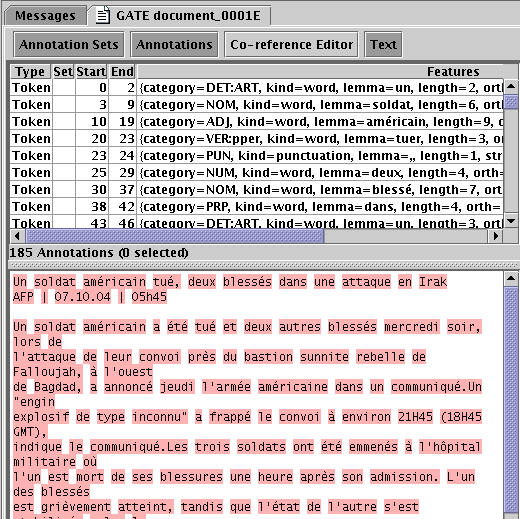
\includegraphics[width=0.5\textwidth]{treetaggertokens.png}
  \caption{A French document processed by the TreeTagger through the Tagger Framework}
  \label{fig:treetagger}
\end{figure}

The tagsets for other languages can be found on the TreeTagger web
site. Figure~\ref{fig:treetagger} shows a screenshot of a French
document processed with the TreeTagger.

\paragraph{Potential Lemma Problems} Sometimes the TreeTagger is either
completely unable to determine the correct lemma, or may return multiple
lemma for a token (separated by a |). In these cases any further processing
that relies on the lemma feature (for example, the flexible gazetteer) may
not function correctly. Both problems can be alleviated somewhat by using
the \verb|resources/TreeTagger/fix-treetagger-lemma.jape| JAPE grammar.
This can be used either as a standalone grammar or as the post-process
initialization feature of the Tagger\_Framework PR.

\subsect[sec:genia-quotes]{GENIA and Double Quotes}
Documents that contain double quote characters can cause problems for 
the GENIA tagger. The issue arises because the in-built GENIA tokenizer
converts double quotes to single quotes in the output which then do not
match the document content, causing the tagger to fail. There are two possible
solutions to this problem.

Firstly you can perform tokenization in GATE and disable the in-built 
GENIA tokenizer. Such a pipeline is provided as an example in the GENIA
resources direcotry; geniatagger-en-no\_tokenization.gapp. However, this may
result in other problems for your subsequent code. If so, you may want to
try the second solution. 

The second solution is to use the GENIA tokenization via the other provided
example pipeline: geniatagger-en-tokenization.gapp. If your documents do not
contain double quotes then this gapp example should work as is. Otherwise,
you must modify the GENIA tagger in order \textit{not} to convert double quotes
to single quotes. Fortunately this is fairly straightforward. In the
resources directory you will find a modified copy of tokenize.cpp from
v3.0.1 of the GENNIA tagger. Simply use this file to replace the copy in the
normal GENIA distribution and recompile. For Windows users, a pre-compiled
binary is also provided -- simply replace your existing binary with this
modified copy.

%%%%%%%%%%%%%%%%%%%%%%%%%%%%%%%%%%%%%%%%%%%%%%%%%%%%%%%%%%%%%%%%%%%%%%%%%%%%%
\sect[sec:parsers:chemistrytagger]{Chemistry Tagger}
%%%%%%%%%%%%%%%%%%%%%%%%%%%%%%%%%%%%%%%%%%%%%%%%%%%%%%%%%%%%%%%%%%%%%%%%%%%%%

This GATE module is designed to tag a number of chemistry items in
running text. Currently the tagger tags compound formulas (e.g.
SO2, H2O, H2SO4 ...) ions (e.g. Fe3+, Cl-) and element names
and symbols (e.g. Sodium and Na). Limited support for compound names
is also provided (e.g. sulphur dioxide) but only when followed by
a compound formula (in parenthesis or commas).

\subsect{Using the Tagger}

The Tagger requires the Creole plugin `Tagger\_Chemistry' to be
loaded.  It requires the following PRs to have been run first:
tokeniser and sentence splitter (the annotation set containing the
Tokens and Sentences can be set using the annotationSetName runtime
parameter).  There are four init parameters giving the locations of 
the two gazetteer list definitions, the element mapping file and the
JAPE grammar used by the tagger (in previous versions of the tagger
these files were fixed and loaded from inside the {\tt ChemTagger.jar}
file).  Unless you know what you are doing you should accept the default
values.

The annotations added to documents are `ChemicalCompound', `ChemicalIon'
and `ChemicalElement' (currently they are always placed in the default
annotation set). By default `ChemicalElement' annotations are removed if they
make up part of a larger compound or ion annotation. This behaviour can be
changed by setting the removeElements parameter to false so that all recognised
chemical elements are annotated.

%%%%%%%%%%%%%%%%%%%%%%%%%%%%%%%%%%%%%%
%\sect[sec:misc-creole:zemanta]{Zemanta Semantic Annotation Service}
%%%%%%%%%%%%%%%%%%%%%%%%%%%%%%%%%%%%%%
%
%There are a number of state-of-the-art methods for semantic annotation and 
%linking to DBpedia (e.g. DBpedia Spotlight, YAGO, and MusicBrainz). In 
%addition, commercial web services such as AlchemyAPI, OpenCalais, and 
%Zemanta are also relevant. A recent evaluation of all state-of-the-art 
%LOD-based methods and tools, showed that DBpedia Spotlight and 
%Zemanta have the best accuracy on annotating texts with the corresponding
%URIs from DBpedia.
%
%Zemanta API (http://developer.zemanta.com) allows application developers 
%to query the Zemanta engine for contextual information about the text 
%that users enter. Given a piece of text, it identifies entities in the 
%text and annotates these entities with their respective URIs in the 
%DBPedia. In GATE, we have provided a wrapper for the Zemanta API. This 
%wrapper, internally, sends the entire document text in a number of 
%batches to the Zemanta service and translates its response into GATE 
%annotations. Further details on the Zemanta service can be found at 
%http://developer.zemanta.com/docs/.
%
%The Zemanta Service PR can be found under the Tagger\_Zemanta plugin in 
%GATE. Below, we describe the various initialization and run time parameters
%of the PR.
%
%\begin{itemize}
%\item \textbf{apiKey}: Since Zemanta is a commercial service, any 
%      non-commercial usage of the service has a constraint on number of 
%      requests that can be made to the Zemanta service.  As on 27 November 
%      2012, this limit is set at one thousand queries per day. In order to 
%      be able to use the PR, you are required to obtain such a key and 
%      provide it to the PR.  The key can be obtained by visiting 
%      http://developer.zemanta.com/docs/ and creating an account on the 
%      website.
%\item \textbf{numberOfSentencesInBatch}: Since Zemanta is a webservice, 
%      only a certain size of text can be sent across for processing. The 
%      number of sentences to be processed in a single batch can be 
%      specified using this PR.  By default, this is set to 10 sentences 
%      per batch.
%\item \textbf{numberOfSentencesInContext}:  Zemanta utilises contextual 
%      information to identy entities and assign each of them a unique URI 
%      (from DBPedia).  This parameter indicates the additional number of 
%      sentences to be sent, both from the left and right contexts, along 
%      with the text to be disambiguated.
%\item \textbf{inputASName}: This is the annotation set where the PR looks
%      for Sentences to be processed.
%\item \textbf{outputASName}: The PR creates annotations of type \textit{Mention}
%      for every entity it identifies in the text.  Such Mention annotations are
%      then stored under the annotation set as specified by the outputASName 
%      parameter.
%\end{itemize}
%
%%%%%%%%%%%%%%%%%%%%%%%%%%%%%%%%%%%%%%%
\sect[sec:misc-creole:lupedia]{Lupedia Semantic Annotation Service}
%%%%%%%%%%%%%%%%%%%%%%%%%%%%%%%%%%%%%%%

Lupedia is a Text Enrichment Service developed by Ontotext. The service 
uses Ontotext's LKB Gazetteer to lookup words against DBpedia and 
LinkedMDB (Linked Movie Database) entities. It supports multiple languages, 
such as English, Italian and French. As part of their service, they provide 
various output filters, weights and heuristics to allow accurate matching. 
The service is aimed at performing lookup but no named entity recognition. 
Ontotext's evaluation of their lupedia API suggests that it is better than 
atleast two other similar services: AlchemyAPI and OpenCalais (see 
http://www.ontotext.com/sites/default/files/publications/lupedia-eval-results.pdf)
for more details on their evaluation.

In GATE, we have developed a wrapper around their online API. The wrapper, 
sends document content to the service and transforms response into GATE 
annotations. The wrapper is called Lupedia Service PR and can be found under 
the Tagger\_Lupedia plugin in GATE. Below, we describe various run time 
parameters of the PR.

\begin{itemize}
\item \textbf{caseSensitive}: This parameter indicates whether the lookup 
      performed against DBPedia and LinkedMDB should be case sensitive or 
      not.
\item \textbf{datasets}: By default, the PR looks up matches of types Person, 
      Event, Place, Organisation and Work and their subtypes as defined in 
      DBPedia ontology.
\item \textbf{keepFirstAndLongestMatch}: This heuristic allows performing 
      longest match. If set to false, it will annotate every possible match.
\item \textbf{keepHighest}: It is possible to have multiple possible URIs for 
      a given string. If this parameter is set to true, only the one with the 
      highest score is kept and remaining low score ones are deleted.
\item \textbf{keepSpecific}: If this parameter is set to true, only the match 
      with most specific URI is preserved.
\item \textbf{lang}: As specified earlier, the PR supports three languages: 
      English, French and Italian.  The lang parameter is to specify the 
      language of the content of the document.
\item \textbf{outputASName}: The PR produces annotations of type Mention. The
      annotations are stored under the annotation set with name specified 
      through this parameter.
\item \textbf{singleGreedyMatch}: Another heuristic which affects the way 
      lookup procedure is carried out. 
\item \textbf{skipShortWords}: If set to true, this parameter ensures that 
      short words (less than 3 characters) are skipped. 
\item \textbf{skipStopWords}: If set to true, stop words are skipped during 
      the lookup procedure.
\item \textbf{threshold}: The PR assigns every match a score. This parameter 
      specifies the minimum score for mentions to be considered as possible 
      candidates. 
\end{itemize}

%%%%%%%%%%%%%%%%%%%%%%%%%%%%%%%%%%%%%%%%%%%%%%%%%%%%%%%%%%%%%%%%%%%%%%%%%%%%%
\sect[sec:misc-creole:textrazor]{TextRazor Annotation Service}
%%%%%%%%%%%%%%%%%%%%%%%%%%%%%%%%%%%%%%%%%%%%%%%%%%%%%%%%%%%%%%%%%%%%%%%%%%%%%

TextRazor (\htlinkplain{http://www.textrazor.com}) is an online service
offering entity and relation annotation, keyphrase extraction, and other
similar services via an HTTP API.  The \verb!Tagger_TextRazor! plugin provides
a PR to access the TextRazor entity annotation API and store the results as
GATE annotations.

The TextRazor Service PR is a simple wrapper around the TextRazor API which
sends the text content of a GATE document to TextRazor and creates one
annotation for each ``entity'' that the API returns.  The PR invokes the
``words'' and ``entities'' \emph{extractors} of the TextRazor API.  The PR has
one initialization parameter:
\begin{description}
\item[apiKey] your TextRazor API key -- to obtain one you must sign up for an
  account at \htlinkplain{http://www.textrazor.com}.
\end{description}

and one (optional) runtime parameter:
\begin{description}
\item[outputASName] the annotation set in which the output annotations should
  be created.  If unset, the default annotation set is used.
\end{description}

The PR creates annotations of type \verb!TREntity! with features
\begin{description}
\item[type] the entity type(s), as class names in the DBpedia ontology.  The
  value of this feature is a \verb!List<String>!.
\item[freebaseTypes] FreeBase types for the entity.  The value of this feature
  is a \verb!List<String>!.
\item[confidence] confidence score (\verb!java.lang.Double!).
\item[ent\_id] canonical ``entity ID'' -- typically the title of the Wikipedia
  page corresponding to the DBpedia instance.
\item[link] URL of the entity's Wikipedia page.
\end{description}

Since the key features are lists rather than single values they may be awkward
to process in downstream components, so a JAPE grammar is provided in the
plugin (\verb!resources/jape/TextRazor-to-ANNIE.jape!) which can be run after
the TextRazor PR to transform key types of TREntity into the corresponding
ANNIE annotation types Person, Location and Organization.

%%%%%%%%%%%%%%%%%%%%%%%%%%%%%%%%%%%%%%%%%%%%%%%%%%%%%%%%%%%%%%%%%%%%%%%%%%%%%
\sect[sec:misc-creole:numbers]{Annotating Numbers}
%%%%%%%%%%%%%%%%%%%%%%%%%%%%%%%%%%%%%%%%%%%%%%%%%%%%%%%%%%%%%%%%%%%%%%%%%%%%%

The Tagger\_Numbers creole repository contains a number of processing resources
which are designed to annotate numbers appearing within documents.
As well as annotating a given span as being a number the PRs also determine the
exact numeric value of the number and add this as a feature of the annotation.
This makes the annotations created by these PRs ideal for building more complex
annotations such as measurements or monetary units.

All the PRs in this plugin produce \texttt{Number} annotations with the
following standard features

\begin{itemize}
\item \textbf{type:} this describes the types of tokens that make up the number,
e.g. roman, words, numbers
\item \textbf{value:} this is the actual value (stored as a Double) of the
number that has been annotated
\end{itemize}

Each PR might also create other features which are described, along with the PR,
in the following sections.

\subsect[sec:misc-creole:numbers:numbers]{Numbers in Words and Numbers}

\begin{table}
\centering
\begin{tabular}{|l|l|}
\hline
String & Value\\
\hline
3\string ^2 & 9\\
101 & 101\\
3,000 & 3000\\
3.3e3 & 3300\\
1/4 & 0.25\\
9\string ^1/2 & 3\\
4x10\string ^3 & 4000\\
5.5*4\string ^5 & 5632\\
thirty one & 31\\
three hundred & 300\\
four thousand one hundred and two & 4102\\
3 million & 3000000\\
f\"{u}nfundzwanzig & 25\\
4 score & 80\\
\hline
\end{tabular}
\caption{Numbers Tagger Examples}
\label{tab:numbers:examples}
\end{table}

The ``Numbers Tagger'' annotates numbers made up from numbers or numeric words.
If that wasn't really clear enough then Table \ref{tab:numbers:examples} shows
numerous ways of representing numbers that can all be annotated by this tagger
(depending upon the configuration files used).

To create an instance of the PR you will need to configure the following
initialization time parameters (sensible defaults are provided):

\begin{itemize}
\item \textbf{configURL:} the URL of the configuration file you wish to use (see
  below for details), defaults to \texttt{resources/languages/all.xml} which
  currently provides support for English, French, German, Spanish and a variety
  of number related Unicode symbols. If you want a single language the you can
  specify the appropriately named file, i.e.
  \texttt{resources/languages/english.xml}.
\item \textbf{encoding:} the encoding of the configuration file, defaults to
  UTF-8
\item \textbf{postProcessURL:} the URL of the JAPE grammar used for
  post-processing -- don't change this unless you know what you are doing!
\end{itemize}

\begin{figure}
\centering
\begin{small}
\begin{verbatim}
<config>
  <description>Basic Example</description>
  <imports>
    <url encoding="UTF-8">symbols.xml</url>
  </imports>
  <words>
    <word value="0">zero</word>
    <word value="1">one</word>
    <word value="2">two</word>
    <word value="3">three</word>
    <word value="4">four</word>
    <word value="5">five</word>
    <word value="6">six</word>
    <word value="7">seven</word>
    <word value="8">eight</word>
    <word value="9">nine</word>
    <word value="10">ten</word>
  </words>
  <multipliers>
    <word value="2">hundred</word>
    <word value="2">hundreds</word>
    <word value="3">thousand</word>
    <word value="3">thousands</word>
    <word value
  </multipliers>
  <conjunctions>
    <word whole="true">and</word>
  </conjunctions>
  <decimalSymbol>.</decimalSymbol>
  <digitGroupingSymbol>,</digitGroupingSymbol>
</config>
\end{verbatim}
\end{small}
\caption{Example Numbers Tagger Config File}
\label{fig:numbers:example}
\end{figure}

The configuration file is an XML document that specifies the words that can be
used as numbers or multipliers (such as hundred, thousand, ...) and conjunctions
that can then be used to combine sequences of numbers together. An example
configuration file can be seen in Figure \ref{fig:numbers:example}. This
configuration file specifies a handful of words and multipliers and a single
conjunction. It also imports another configuration file (in the same format)
defining Unicode symbols.

The words are self-explanatory but the multipliers and conjunctions need further
clarification.

There are three possible types of multiplier:

\begin{itemize}
\item \textbf{e}: This is the default multiplier type (i.e. is used if the type
is missing) and signifies base 10 exponential notation. For example, if the specified
value is 2 then this is expanded to $\times 10^2$, hence converting the text ``3 hundred'' into
$3 \times 10^2$ or 300.
\item \textbf{/}: This type allows you to define fractions. For example you would define a half using the value 2 (i.e.
you divide by 2). This allows text such as ``three halves'' to be normalized to 1.5 (i.e. $3/2$). Note that
you can also use this type of multiplier to specify multiples greater than one. For example, the text ``four score''
should be normalized to 80 as a score represents 20 years. To specifiy such a multiplier we use the fraction type
with a value of 0.05. This leads to normalized value being calculated as $4/0.05$ which is 80. To determine the
value use the simple formula $(100/multipe)/100$
\item \textbf{\^}: Multipliers of this type allow you to specify powers. For example, you could define ``squared'' with
a value of 2 to allow the text ``three squared'' to be normalized to the number 9.
\end{itemize}

In English conjunctions
are whole words, that is they require white space on either side of them, e.g.
three hundred and one. In other languages, however, numbers can be joined into a
single word using a conjunction. For example, in German the conjunction `und'
can appear in a number without white space, e.g. twenty one is written as
einundzwanzig. If the conjunction is a whole word, as in English, then the whole
attribute should be set to true, but for conjunctions like `und' the attribute
should be set to false.

In order to support different number formats the symbols used to group numbers
and to represent the decimal point can also be configured. These are optional
elements in the XML configuration file which if not supplied default to a comma
for the digit group symbol and a full stop for the decimal point. Whilst these
are appropriate for many languages if you wanted, for example, to parse
documents written in Bulgarian you would want to specify that the decimal symbol
was a command and the grouping symbol was a space in order to recognise numbers
such as 1 000 000,303.

Once created an instance of the PR can then be configured using the following
runtime parameters:

\begin{itemize}
\item \textbf{allowWithinWords:} digits can often occur within words (for
  example part numbers, chemical equations etc.) where they should not be
  interpreted as numbers. If this parameter is set to true then these instances
  will also be annotated as numbers (useful for annotating money and
  measurements where spaces are often omitted), however, the parameter defaults
  to false.
\item \textbf{annotationSetName:} the annotation set to use as both input and
  output for this PR (due to the way this PR works the two sets have to be the
  same)
\item \textbf{failOnMissingInputAnnotations:} if the input annotations (Tokens
  and Sentences) are missing should this PR fail or just not do anything,
  defaults to true to allow  obvious mistakes in pipeline configuration to be
  captured at an early stage.
\item \textbf{useHintsFromOriginalMarkups:} often the original markups will
  provide hints that may be useful for correctly interpreting numbers within
  documents  (i.e. numeric powers may be in $<$sup$><$/sup$>$ tags), if this
  parameter is set to true then these hints will be used to help parse the
  numbers, defaults to true.
\end{itemize}

There are no extra annotation features which are specific to this numbers PR.
The \texttt{type} feature can take one of three values based upon the text that
is annotated; words, numbers, wordsAndNumbers.

\subsect[sec:misc-creole:numbers:roman]{Roman Numerals}

The ``Roman Numerals Tagger'' annotates Roman numerals appearing in the document. The tagger is configured using the following runtime parameters:

\begin{itemize}
\item \textbf{allowLowerCase:} traditionally Roman numerals must be all in uppercase. Setting this parameter to false, however, allows Roman numerals written in lowercase
  to also be annotated. This parameter defaults to false.
\item \textbf{maxTailLength:} Roman numerals are often used in labelling sections, figures, tables etc. and in such cases can be followed by additional information. For
  example, Table IVa, Appendix IIIb. These characters are referred to as the tail of the number and this parameter constrains the number of characters that can appear. The default value is 0 in which case strings such as 'IVa' would not be annotated in any way.
\item \textbf{outputASName:} the name of the annotation set in which the Number annotations should be created.
\end{itemize}

As well as the normal Number annotation features (the \texttt{type} feature will
always take the value `roman') Roman numeral annotations also include the
following features:

\begin{itemize}
\item \textbf{tail:} contains the tail, if any, that appears after the Roman numeral.
\end{itemize}

%%%%%%%%%%%%%%%%%%%%%%%%%%%%%%%%%%%%%%%%%%%%%%%%%%%%%%%%%%%%%%%%%%%%%%%%%%%%%
\sect[sec:misc-creole:measurements]{Annotating Measurements}
%%%%%%%%%%%%%%%%%%%%%%%%%%%%%%%%%%%%%%%%%%%%%%%%%%%%%%%%%%%%%%%%%%%%%%%%%%%%%

Measurements mentioned in text documents can be difficult to accurately deal
with. As well as the numerous ways in which numeric values can be written each
type of measurement (distance, area, time etc.) can be written using a variety
of different units.
For example, lengths can be measured in metres, centimetres, inches, yards,
miles, furlongs and chains, to mention just a few.
Whilst measurements may all have different units and values they can, in theory
be compared to one another. Extracting, normalizing and comparing measurements
can be a useful IE process in many different domains. The Measurement Tagger
(which can be found in the Tagger\_Measurements plugin) attempts to provide such
annotations for use within IE applications.

The Measurements Tagger uses a parser based upon a modified version of the
\htlink{http://units-in-java.sourceforge.net/}{Java port} of the
\htlink{http://www.gnu.org/software/units/}{GNU Units} package. This allows us
to not only recognise and annotation spans of text as being a measurement but
also to normalize the units to allow for easy comparison of different
measurement values.

This PR actually produces two different annotations; Measurement and Ratio.

Measurement annotations represent measurements that involve a unit, e.g. 3mph,
three pints, 4 m$^3$. Single measurements (i.e. those not referring to a range
or interval) are referred to as scalar measurements and have the following
features:
\begin{itemize}
\item \texttt{type}: for scalar measurements is always \texttt{scalar}
\item \texttt{unit}: the unit as recognised from the text. Note that this won't
  necessarily be the annotated text. For example, an annotation spanning the
 text ``three miles'' would have a \texttt{unit} feature of ``mile''.
\item \texttt{value}: a Double holding the value of the measurement (this
  usually comes directly from the \texttt{value} feature of a Number
 annotation).
\item \texttt{dimension}: the measurements dimension, e.g. speed, volume, area,
  length, time etc. 
\item \texttt{normalizedUnit}: to enable measurements of the same dimension but
  specified in different units to be compared the PR reduces all units to their
  base form. A base form usually consists of a combination of
  \htlink{http://en.wikipedia.org/wiki/International\string_System\string_of\string_Units}{SI units}.
  For example, centimetre, mm, and kilometre are all normalized to m (for
  metre).
\item \texttt{normalizedValue}: a Double instance holding the normalized value,
  such that the combination of the normalized value and normalized unit
  represent the same measurement as the original value and unit. 
\item \texttt{normalized}: a String representing the normalized measurement
  (usually a simple space separated concatenation of the normalized value and
  unit).
\end{itemize}

Annotations which represent an interval or range have a slightly different set
of features. The \texttt{type} feature is set to \texttt{interval}, there is no
\texttt{normalized} or \texttt{unit} feature and the value features (included
the normalized version) are replaced by the following features, the values of
which are simply copied from the Measurement annotations which mark the
boundaries of the interval.

\begin{itemize}
\item \texttt{normalizedMinValue}: a Double representing the minimum normalized
  number that forms part of the interval. 
\item \texttt{normalizedMaxValue}: a Double representing the minimum normalized
  number that forms part of the interval.
\end{itemize}

Interval annotations do not replace scalar measurements and so multiple
Measurement annotations may well overlap. They can of course be distinguished by
the \texttt{type} feature.

As well as Measurement annotations the tagger also adds Ratio annotations to
documents. Ratio annotations cover measurements that do not have a unit.
Percentages are the most common ratios to be found in documents, but also
amounts such as ``300 parts per million'' are annotated.

A Ratio annotation has the following features:

\begin{itemize}
\item \texttt{value}: a Double holding the actual value of the ratio. For
  example, 20\% will have a value of 0.2.
\item \texttt{numerator}: the numerator of the ratio. For example, 20\% will
  have a numerator of 20.
\item \texttt{denominator}: the denominator of the ratio. For example, 20\% will
  have a denominator of 100.
\end{itemize}

An instance of the measurements tagger is created using the following
initialization parameters:

\begin{itemize}
\item \textbf{commonURL:} this file defines units that are also common words and
  so should not be annotated as a measurement unless they form a compound unit
  involving two or more unit symbols. For example, C is the accepted
  abbreviation for coulomb but often appears in documents as part of a reference
  to a table or figure, i.e. Figure 3C, which should not be annotated as a
  measurement. The default file was hand tuned over a large patent corpus but
  may need to be edited when used with different domains.
\item \textbf{encoding:} the encoding to use when reading both of the
  configuration files, defaults to UTF-8.
\item \textbf{japeURL:} the URL of the JAPE grammar that drives the measurement
  parser. Unless you really know what you are doing, the value of this parameter
  should not be changed.
\item \textbf{locale:} the locale to use when parsing the units definition file,
  defaults to en\_GB.
\item \textbf{unitsURL:} the URL of the main unit definition file to use. This
  should be in the same
\htlink{http://www.gnu.org/software/units/manual/html\string_node/Defining-new-units.html}{format} as accepted by the GNU Units package.
\end{itemize}

The PR does not attempt to recognise or annotate numbers, instead it relies on
Number annotations being present in the document. Whilst these annotations could
be generated by any resource executed prior to the measurements tagger, we
recommend using the Numbers Tagger described in Section
\ref{sec:misc-creole:numbers}. If you choose to produce Number annotations in
some other way note that they must have a \texttt{value} feature containing a
Double representing the value of the number. An example GATE application,
showing how to configure and use the two PRs together, is provided with the
measurements plugin.

Once created an instance of the tagger can be configured using the following
runtime parameters:

\begin{itemize}
\item \textbf{consumeNumberAnnotations:} if true then Number annotations used to
  find measurements will be consumed and removed from the document, defaults to
  true.
\item \textbf{failOnMissingInputAnnotations:} if the input annotations (Tokens)
  are missing should this PR fail or just not do anything, defaults to true to
  allow obvious mistakes in pipeline configuration to be captured at an early
  stage. 
\item \textbf{ignoredAnnotations:} a list of annotation types in which a
  measurement can never occur, defaults to a set containing Date and Money.
\item \textbf{inputASName:} the annotation set used as input to this PR.
\item \textbf{outputASName:} the annotation set to which new annotations will
  be added.
\end{itemize}

The ability to prevent the tagger from annotating measurements which occur
within other annotations is a very useful feature. The runtime parameters,
however, only allow you to specify the names of annotations and not to restrict
on feature values or any other information you may know about the documents
being processed.
Internally ignoring sections of a document is controlled by adding
CannotBeAMeasurement annotations that span the text to be ignored. If you need
greater control over the process than the \texttt{ignoredAnnotations} parameter
allows then you can create CannotBeAMeasurement annotations prior to running the
measurement tagger, for example a JAPE grammar placed before the tagger in the
pipeline. Note that these annotations will be deleted by the measurements tagger
once processing has completed.

%%%%%%%%%%%%%%%%%%%%%%%%%%%%%%%%%%%%%%%%%%%%%%%%%%%%%%%%%%%%%%%%%%%%%%%%%%%%%
\sect[sec:misc-creole:datenormalizer]{Annotating and Normalizing Dates}
%%%%%%%%%%%%%%%%%%%%%%%%%%%%%%%%%%%%%%%%%%%%%%%%%%%%%%%%%%%%%%%%%%%%%%%%%%%%%

Many information extraction tasks benefit from or require the extraction of
accurate date information. While ANNIE (Chapter \ref{chap:annie}) does produce
Date annotations no attempt is made to normalize these dates, i.e. to firmly
fix all dates, even partial or relative ones, to a timeline using a common
date representation. The PR in the Tagger\_DateNormalizer plugin attempts
to fill this gap by normalizing dates against the date of the document (see
below for details on how this is determined) in order to tie each Date
annotation to a specific date. This includes normalizing dates such as
April 1st, today, yesterday, and next Tuesday, as well as converting
fully specified dates (ones in which the day, month and year are
specified) into a common format.

Different cultures/countries have different conventions for writing dates, as
well as different languages using different words for the days of the week and
the months of the year. The parser underlying this PR makes use of the
\textit{locale-specific} information when parsing documents. When initializing
an instance of the Date Normalizer you can specify the locale to use using
ISO language and country codes along with Java specific variants (for details
of these codes see the Java
\htlink{http://docs.oracle.com/javase/6/docs/api/java/util/Locale.html}{Locale documentation}).
So for example, to specify British English (which means the day usually comes
before the month in a date) use \texttt{en\_GB}, or for American English (where
the month usually appears before the day in a date) specify \texttt{en\_US}.
If you need to override the locale on a document basis then you can do this by
setting a document feature called locale to a string encoded as above. If neither
the initialization parameter or document feature are present or do not represent
a valid locale then the default locale of the JVM running GATE will be used.

Once initialized and added to a pipeline the Date Normalizer has the following
runtime parameters that can be used to control it's behaviour.

\begin{itemize}
\item \textbf{annotationName:} the annotation type created by this PR, defaults
  to Date.
\item \textbf{dateFormat:} the format that dates should be normalized to. The
  format of this parameter is the same as that use by the Java
  \htlink{http://docs.oracle.com/javase/6/docs/api/java/text/SimpleDateFormat.html}{SimpleDateFormat}
  whose documentation describes the full range of possible formats (note you
  must use MM for month and not mm). This defaults to dd/MM/yyyy.
  Note that this parameter is only required if the numericOuput parameter is set to false.
\item \textbf{failOnMissingInputAnnotations:} if the input annotations (Tokens)
  are missing should this PR fail or just not do anything, defaults to true to
  allow obvious mistakes in pipeline configuration to be captured at an early stage.
\item \textbf{inputASName:} the annotation set used as input to this PR.
\item \textbf{normalizedDocumentFeature:} if set then the normalized version
  of the document date will be stored in a document feature with this name.
  This parameter defaults to normalized-date although it can be left blank
  to suppress storage of the document date.  
\item \textbf{numericOutput:} if true then instead of formatting the normalized
  dates as String features of the Date annotations they are instead converted
  into a numeric representation. Specifically the first converted to the form
  yyyyMMdd and then cast to a Double. This is useful as dates can then be sorted
  numerical (which is fast) into order. If false then the formatting string
  in the dateFormat parameter is used instead to create a string representation.
  This defaults to false.
\item \textbf{outputASName:} the annotation set to which new annotations will
  be added.
\item \textbf{sourceOfDocumentDate:} this parameter is a list of the names of
  annotations, annotation features (encoded as Annotation.feature), and document
  features to inspect when trying to determine the date of the document. The PR
  works through the list getting the text of feature or under the annotation
  (if no feature is specified) and then parsing this to find a fully specified
  date, i.e. one where the day, month and year are all present. Once a date is
  found processing of the list stops and the date is used as the date of the
  document. If you specify an annotation that can occur multiple times in a
  document then they are sorted based on a numeric priority feature (which defaults
  to 0) or their order within the document. The idea here is that there are 
  multiple ways in which to determine the date of a document but most are domain
  specific and this allows previous PRs in an application to determine the
  document date. This defaults to an empty list which is taken to assume that
  the document was written on the day it is being processed. The same assumption
  applies if no fully-specified date can be found once the whole list has
  been processed. Note that a common mistake is to think you can use a date
  annotated by this PR as the document date. The document date is determined before
  the document is processed, so any annotation you wish to use to represent the
  document date must exist before this PR executes.
\end{itemize}

It is important to note that rather this plugin creates new Date annotations
and so if you run it in the same pipeline as the ANNIE NE Transducer you will
likely end up with overlapping Date annotations. Depending on your needs it
may be that you need a JAPE grammar to delete ANNIE Date annotations before
running this PR. In practice we have found that the Date annotations added
by ANNIE can be a good source of document dates and so a JAPE grammar that
uses ANNIE Dates to add new DocumentDate annotations and to delete other
Date annotations can be a useful step before running this PR.

The annotations created by this PR have the following features:

\begin{itemize}
\item \textbf{normalize:} the normalized date in the format specified through the
relevant runtime parameters of the PR.
\item \textbf{inferred:} an integer which specifies which specifes which parts of the
date had to be inferred. The value is actually a bit mask created from the following
flagd: day = 1, month = 2, and year = 4. You can find which (if any) flags are set
by using the code \texttt{(inferred \& FLAG) == FLAG}, i.e. to see if the day of the month
had to be inferred you would do \texttt{(inferred \& 1) == 1}.
\item \textbf{complete:} if no part of the date had to be inferred (i.e. inferred = 0) then
this will be true, false otherwise.
\item \textbf{relative:} can take the values past, present or future to show how this
specific date relates to the document date.
\end{itemize}

%%%%%%%%%%%%%%%%%%%%%%%%%%%%%%%%%%%%%%%%%%%%%%%%%%%%%%%%%%%%%%%%%%%%%%%%%%%%%
\sect[sec:parsers:stemmer]{Snowball Based Stemmers}
%%%%%%%%%%%%%%%%%%%%%%%%%%%%%%%%%%%%%%%%%%%%%%%%%%%%%%%%%%%%%%%%%%%%%%%%%%%%%

The stemmer plugin, `Stemmer\_Snowball', consists of a set of stemmers PRs for
the following 11 European languages: Danish, Dutch, English, Finnish, French,
German, Italian, Norwegian, Portuguese, Russian, Spanish and Swedish. These take
the form of wrappers for the Snowball stemmers freely available from
\htlinkplain{http://snowball.tartarus.org}. Each Token is annotated with a new
feature `stem', with the stem for that word as its value. The stemmers should be
run as other PRs, on a document that has been tokenised.

There are three runtime parameters which should be set prior to executing 
the stemmer on a document.

\begin{itemize}
\item annotationType: This is the type of annotations that represent tokens
          in the document.  Default value is set to `Token'.

\item annotationFeature: This is the name of a feature that contains tokens'
          strings. The stemmer uses value of this feature as a string to be 
          stemmed.  Default value is set to `string'.

\item annotationSetName: This is where the stemmer expects the 
         annotations of type as specified in the annotationType parameter to be.

\end{itemize}

\subsect{Algorithms}

The stemmers are based on the Porter stemmer for English \cite{Porter80}, with
rules implemented in Snowball e.g.
\begin{small}
\begin{verbatim}
define Step_1a as
( [substring] among (
 'sses' (<-'ss')
'ies' (<-'i')
'ss' () 's'  (delete)
 )
 \end{verbatim}
\end{small}

%%%%%%%%%%%%%%%%%%%%%%%%%%%%%%%%%%%%%%%%%%%%%%%%%%%%%%%%%%%%%%%%%%%%%%%%%%%%
\sect[sec:parsers:morpher]{GATE Morphological Analyzer}
%%%%%%%%%%%%%%%%%%%%%%%%%%%%%%%%%%%%%%%%%%%%%%%%%%%%%%%%%%%%%%%%%%%%%%%%%%%%

The Morphological Analyser PR can be found in the Tools plugin. It
takes as input a tokenized GATE document. Considering one token and
its part of speech tag, one at a time, it identifies its lemma and an
affix. These values are than added as features on the Token
annotation. Morpher is based on certain regular expression rules.
These rules were originally implemented by \textit{Kevin Humphreys} in
GATE1 in a programming language called \textit{Flex}. Morpher has a
capability to interpret these rules with an extension of allowing
users to add new rules or modify the existing ones based on their
requirements. In order to allow these operations with as little effort
as possible, we changed the way these rules are written. More
information on how to write these rules is explained later in
Section \ref{sec:parsers:morpher:rules}.

Two types of parameters, Init-time and run-time, are required to
instantiate and execute the PR.

\begin{itemize}

\item {rulesFile (Init-time)} The rule file has several regular expression patterns.
Each pattern has two parts, L.H.S. and R.H.S. L.H.S. defines the regular
expression and R.H.S. the function name to be called when the pattern matches
with the word under consideration. Please see \ref{sec:parsers:morpher:rules} for more
information on rule file.

\item {caseSensitive (init-time)} By default, all tokens under consideration are
converted into lowercase to identify their lemma and affix. If the user selects
\textit{caseSensitive} to be \textit{true}, words are no longer converted into
lowercase.

\item{document (run-time)} Here the document must be an instance of a GATE
document.

\item{affixFeatureName (run-time)} Name of the feature that should hold the affix value.

\item{rootFeatureName (run-time)} Name of the feature that should hold the root value.

\item{annotationSetName (run-time)} Name of the annotationSet that contains Tokens.

\item{considerPOSTag (run-time)} Each rule in the rule file has a separate tag, which specifies which rule to consider with what part-of-speech tag. If this option is set to false, all rules are considered and matched with all words. This option is very useful. For example if the word under consideration is "singing".  "singing" can be used as a noun as well as a verb. In the case where it is identified as a verb, the lemma of the same would be "sing" and the affix "ing", but otherwise there would not be any affix.

\item{failOnMissingInputAnnotations (run-time)} If set to true (the default) the PR
will terminate with an Exception if none of the required input Annotations are found in 
a document. If set to false the PR will not terminate and instead log a 
single warning message per session and a debug message per document that has no
input annotations.

\end{itemize}

%%%%%%%%%%%%%%%%%%%%%%%%%%%%%%%%%%%%%%%%%%%%%%%%%%%%%%%%%%%%%%%%%%%%%%%%%%%%
\subsect[sec:parsers:morpher:rules]{Rule File}
%%%%%%%%%%%%%%%%%%%%%%%%%%%%%%%%%%%%%%%%%%%%%%%%%%%%%%%%%%%%%%%%%%%%%%%%%%%%

GATE provides a default rule file, called \textit{default.rul}, which
is available under the \textit{gate/plugins/Tools/morph/resources}
directory. The rule file has two sections.

\begin{enumerate}
\item{Variables}
\item{Rules}
\end{enumerate}

\subsubsect{Variables}

The user can define various types of variables under the section
\textit{defineVars}. These variables can be used as part of the regular
expressions in rules. There are three types of variables:

\begin{enumerate}

\item{Range} With this type of variable, the user can specify the range of
characters. e.g. A $==>$ [-a-z0-9]

\item{Set} With this type of variable, user can also specify a set of
characters, where one character at a time from this set is used as a value for
the given variable. When this variable is used in any regular expression, all
values are tried one by one to generate the string which is compared with
the contents
of the document. e.g. A $==>$ [abcdqurs09123]

\item{Strings} Where in the two types explained above, variables can hold only
one character from the given set or range at a time, this allows specifying
strings as possibilities for the variable. e.g. A $==>$ `bb' OR `cc' OR `dd'

\end{enumerate}


\subsubsect{Rules}

All rules are declared under the section \textit{defineRules}. Every rule has
two parts, LHS and RHS. The LHS specifies the regular expression and the RHS
the function to be called when the LHS matches with the given word. `$==>$' is
used as delimiter between the LHS and RHS.

The LHS has the following syntax:

$<"*" $|$ "verb" $|$ "noun"><regular expression>$.

User can specify which rule to be considered when the word is identified as
`verb' or `noun'. `*' indicates that the rule should be considered for all
part-of-speech tags. If the part-of-speech should be used to decide if the rule
should be considered or not can be enabled or disabled by setting the value of
\textit{considerPOSTags} option. Combination of any string along with any of the
variables declared under the \textit{defineVars} section and also the Kleene
operators, `+' and `*', can be used to generate the regular expressions. Below
we give few examples of L.H.S. expressions.

\begin{itemize}

\item{$<$verb$>$"bias"}

\item{$<$verb$>$"canvas"\{ESEDING\}} "ESEDING" is a variable defined under the
\textit{defineVars} section. Note: variables are enclosed with "\{" and "\}".

\item{$<$noun$>$(\{A\}*"metre")} "A" is a variable followed by the Kleene operator "*", which means "A" can occur zero or more times.

\item{$<$noun$>$(\{A\}+"itis")} "A" is a variable followed by the Kleene operator "+", which means "A" can occur one or more times.

\item{$<*>$"aches"} "$<*>$" indicates that the rule should be considered for all part-of-speech tags.

\end{itemize}


On the RHS of the rule, the user has to specify one of the functions
from those listed below. These rules are hard-coded in the Morph PR in GATE and
are invoked if the regular expression on the LHS matches with any
particular word.

\begin{itemize}
\item{stem(\textit{n}, \textit{string}, \textit{affix})} Here,
    \begin{itemize}
    \item{\textit{n}} = number of characters to be truncated from the end of the string.
    \item{\textit{string}} = the string that should be concatenated after the word to produce the root.
    \item{\textit{affix}} = affix of the word
    \end{itemize}

\item{irreg\_stem(\textit{root}, \textit{affix})} Here,
    \begin{itemize}
    \item{\textit{root}} = root of the word
    \item{\textit{affix}} = affix of the word
    \item{null\_stem()} This means words are themselves the base forms and
    should not be analyzed.
    \end{itemize}
\item{semi\_reg\_stem(\textit{n},\textit{string})}
    \textit{semir\_reg\_stem} function is used with the regular expressions
    that end with any of the \{EDING\} or \{ESEDING\} variables defined
    under the variable section. If the regular expression matches with the
    given word, this function is invoked, which returns the value of
    variable (i.e. \{EDING\} or \{ESEDING\}) as an affix. To find a lemma of
    the word, it removes the \textit{n} characters from the back of the word
    and adds the \textit{string} at the end of the word.
\end{itemize}

%%%%%%%%%%%%%%%%%%%%%%%%%%%%%%%%%%%%%%%%%%%%%%%%%%%%%%%%%%%%%%%%%%%%%%%%%%%%%
\sect[sec:misc-creole:flexexport]{Flexible Exporter}
%%%%%%%%%%%%%%%%%%%%%%%%%%%%%%%%%%%%%%%%%%%%%%%%%%%%%%%%%%%%%%%%%%%%%%%%%%%%%

The Flexible Exporter enables the user to save a document (or corpus)
in its original format with added annotations. The user can select the
name of the annotation set from which these annotations are to be
found, which annotations from this set are to be included, whether
features are to be included, and various renaming options such as
renaming the annotations and the file.

At load time, the following parameters can be set for the flexible
exporter:
\begin{itemize}
\item includeFeatures - if set to true, features are included with the
annotations exported; if false (the default status), they are not.

\item useSuffixForDumpFiles - if set to true  (the default status),
the output files have the suffix defined in suffixForDumpFiles; if
false, no suffix is defined, and the output file simply overwrites the
existing file (but see the outputFileUrl runtime parameter for an
alternative).

\item suffixForDumpFiles - this defines the suffix if
useSuffixForDumpFiles is set to true. By default the suffix is .gate.

\item useStandOffXML - if true then the format will be the GATE XML format
that separates nodes and annotations inside the file which allows
overlapping annotations to be saved.

\end{itemize}
%%%

The following runtime parameters can also be set (after the file has
been selected for the application):

%%%
\begin{itemize}

\item annotationSetName - this enables the user to specify the name of
the annotation set which contains the annotations to be exported. If
no annotation set is defined, it will use the Default annotation set.

\item annotationTypes - this contains a list of the annotations to be
exported. By default it is set to Person, Location and Date.

\item dumpTypes - this contains a list of names for the exported
annotations. If the annotation name is to remain the same, this list
should be identical to the list in annotationTypes. The list of
annotation names must be in the same order as the corresponding
annotation types in annotationTypes.

\item outputDirectoryUrl - this enables the user to specify the export directory
where the file is exported with its original name and an extension (provided as
a parameter) appended at the end of filename. Note that you can also save a
whole corpus in one go. If not provided, use the temporary directory.

\end{itemize}

%%%%%%%%%%%%%%%%%%%%%%%%%%%%%%%%%%%%%%%%%%%%%%%%%%%%%%%%%%%%%%%%%%%%%%%%%%%%%
\sect[sec:misc-creole:confexport]{Configurable Exporter}
%%%%%%%%%%%%%%%%%%%%%%%%%%%%%%%%%%%%%%%%%%%%%%%%%%%%%%%%%%%%%%%%%%%%%%%%%%%%%

The Configurable Exporter allows the user to export arbitrary
annotation texts and feature values according to a format specified in
a configuration file. It is written with machine learning in mind,
where features might be required in a comma separated format or
similar, though it could be equally well applied to any purpose where
data are required in a spreadsheet format or a simple format for
further processing. An example of the kind of output that can be
obtained using the PR is given below, although significant variation
on the theme is possible, showing typical instance IDs, classes and
attributes:

\begin{verbatim}

10000004, A, "Some text .."
10000005, A, "Some more text .."
10000006, B, "Further text .."
10000007, B, "Additional text .."
10000008, B, "Yet more text .."

\end{verbatim}

Central to the PR is the concept of an instance; each line of output
will relate to an instance, which might be a document for example, or
an annotation type within a GATE document such as a sentence, tweet,
or indeed any other annotation type. Instance is specified as a
runtime parameter (see below). Whatever you want one per line of, that
is your instance.

The PR has one required initialisation parameter, which is the
location of the configuration file. If you edit your configuration
file, you must reinitialise the PR. The configuration file comprises a
single line specifying the output format. Annotation and feature names
are surrounded by triple angle brackets, indicating that they are to
be replaced with the annotation/feature. The rest of the text in the
configuration file is passed unchanged into the output file. Where an
annotation type is specified without a feature, the text spanned by
that annotation will be used. Dot notation is used to indicate that a
feature value is to be used. The example output given above might be
obtained by a configuration file something like this, in which index,
class and content are annotation types:

\begin{verbatim}

{index}, {class}, "{content}"

\end{verbatim}

Alternatively, in this example, class is a feature on the instance
annotation:

\begin{verbatim}

{index}, {instance.class}, "{content}"

\end{verbatim}

Runtime parameters are as follows:

\begin{itemize}

\item{inputASName - this is the annotation set which will be used to 
create the export file. All annotations must be in this set, both 
instance annotations and export annotations. If left blank, the default 
annotation set will be used.}

\item{instanceName - this is the annotation type to be used as instance. 
If left blank, the document will be used as instance.}

\item{outputURL - this is the location of the output file to which the 
data will be exported. If left blank, data will be output to the 
messages tab/standard out.}

\end{itemize}

Note that where more than one annotation of the specified type occurs
within the span of the instance annotation, the first will be used to
create the output. It is not currently supported to output more than
one annotation of the same type per instance. If you need to export,
for example, all the words in the sentence, then you would have to
export the sentence rather than the individual words.


%%%%%%%%%%%%%%%%%%%%%%%%%%%%%%%%%%%%%%%%%%%%%%%%%%%%%%%%%%%%%%%%%%%%%%
\sect[sec:misc-creole:ast]{Annotation Set Transfer}
%%%%%%%%%%%%%%%%%%%%%%%%%%%%%%%%%%%%%%%%%%%%%%%%%%%%%%%%%%%%%%%%%%%

The Annotation Set Transfer allows copying or moving annotations to
a new annotation set if they lie between the beginning and the end
of an annotation of a particular type (the covering annotation). For
example, this can be used when a user only wants to run a processing
resource over a specific part of a document, such as the Body of an
HTML document. The user specifies the name of the annotation set and
the annotation which covers the part of the document they wish to
transfer, and the name of the new annotation set. All the other
annotations corresponding to the matched text will be transferred to
the new annotation set. For example, we might wish to perform named
entity recognition on the body of an HTML text, but not on the
headers. After tokenising and performing gazetteer lookup on the whole
text, we would use the Annotation Set Transfer to transfer those
annotations (created by the tokeniser and gazetteer) into a new
annotation set, and then run the remaining NE resources, such as the
semantic tagger and coreference modules, on them.

The Annotation Set Transfer has no loadtime parameters. It has the
following runtime parameters:
%
\begin{itemize}
\item
\texttt{inputASName} - this defines the annotation set from which annotations will be
transferred (copied or moved). 
If nothing is specified, the Default annotation set will
be used.
\item
\texttt{outputASName} - this defines the annotation set to which the annotations
will be transferred. This default value for this parameter is `Filtered'. If it 
is left blank the Default annotation set will be used.
\item
\texttt{tagASName} - this defines the annotation set which contains the
annotation covering the relevant part of the document to be
transferred. This default value for this parameter is `Original markups'. If it 
is left blank the Default annotation set will be used.
\item
\texttt{textTagName} - this defines the type of the annotation covering
the annotations to be transferred. The default value for this parameter is
`BODY'. If this is left blank, then all annotations from the inputASName 
annotation set will be transferred. If more than one covering annotation 
is found, the annotation covered by each of them will be transferred. If no 
covering annotation is found, the processing depends on the \texttt{copyAllUnlessFound} 
parameter (see below).
\item
\texttt{copyAnnotations} - this specifies whether the annotations should 
be moved or copied. The default value \texttt{false} will move annotations,
removing them from the \texttt{inputASName} annotation set. If set to 
\texttt{true} the annotations will be copied.
\item 
\texttt{transferAllUnlessFound} - this specifies what should happen if no covering
annotation is found. The default value is \texttt{true}. In this case, all
annotations will be copied or moved (depending on the setting of parameter
\texttt{copyAnnotations}) if no covering annotation is found.
If set to \texttt{false}, no annotation will be copied or moved.
\item \texttt{annotationTypes} - if annotation type names are specified
for this list, only candidate annotations of those types will be
transferred or copied. If an entry in this list is specified in the 
form \texttt{OldTypeName=NewTypeName}, then annotations of type 
\texttt{OldTypeName} will be selected for copying or transfer and 
renamed to \texttt{NewTypeName} in the output annotation set.
\end{itemize}
%
For example, suppose we wish to perform named entity recognition on
only the text covered by the BODY annotation from the Original Markups
annotation set in an HTML document. We have to run the gazetteer and
tokeniser on the entire document, because since these resources do not
depend on any other annotations, we cannot specify an input annotation
set for them to use. We therefore transfer these annotations to a new
annotation set (Filtered) and then perform the NE recognition over these
annotations, by specifying this annotation set as the input annotation set
for all the following resources. In this example, we would set the following
parameters (assuming that the annotations from the tokenise and
gazetteer are initially placed in the Default annotation set).
\begin{itemize}
\item inputASName: Default
\item outputASName: Filtered
\item tagASName: Original markups
\item textTagName: BODY
\item copyAnnotations: true or false (depending on whether we want to keep
the Token and Lookup annotations in the Default annotation set)
\item copyAllUnlessFound: true
\end{itemize}

The AST PR makes a shallow copy of the feature map for each transferred
annotation, i.e. it creates a new feature map containing the same keys and
values as the original.  It does \emph{not} clone the feature values
themselves, so if your annotations have a feature whose value is a collection
and you need to make a deep copy of the collection value then you will not be
able to use the AST PR to do this.  Similarly if you are copying annotations
and \emph{do} in fact want to share the same feature map between the source and
target annotations then the AST PR is not appropriate.  In these sorts of cases
a JAPE grammar or Groovy script would be a better choice.



%%%%%%%%%%%%%%%%%%%%%%%%%%%%%%%%%%%%%%%%%%%%%%%%%%%%%%%%%%%%%%%%%%%%%%%%%%%%%
\sect[sec:misc-creole:schemaenforcer]{Schema Enforcer}
%%%%%%%%%%%%%%%%%%%%%%%%%%%%%%%%%%%%%%%%%%%%%%%%%%%%%%%%%%%%%%%%%%%%%%%%%%%%%

One common use of the Annotation Set Transfer (AST) PR (see Section \ref{sec:misc-creole:ast})
is to create a `clean' or final annotation set for a GATE application, i.e. an annotation set containing
only those annotations which are required by the application without any temporary or intermediate
annotations which may also have been created. Whilst really useful the AST suffers from two
problems 1) it can be complex to configure and 2) it offers no support for modifying or removing
features of the annotations it copies.

Many GATE applications are developed through a process which starts with experts
manually annotating documents in order for the application developer to understand what
is required and which can later be used for testing and evaluation. This is usually done using either
\htlink{http://gate.ac.uk/teamware/}{GATE Teamware} or within GATE Developer using
the Schema Annotation Editor (Section \ref{sec:developer:schemaannotationeditor}). Either
approach requires that each of the annotation types being created is described by an
XML based Annotation Schema. The Schema Enforcer (part of the Schema\_Tools plugin) uses these
same schemas to create an annotation set, the contents of which, strictly matches the provided schemas.

The Schema Enforcer will copy an annotation if and only if....
\begin{itemize}
\item the type of the annotation matches one of the supplied schemas
\item all required features are present and valid (i.e. meet the requirements
    for being copied to the 'clean' annotation)
\end{itemize}

Each feature of an annotation is copied to the new annotation if and only if....
\begin{itemize}
\item the feature name matches a feature in the schema describing the annotation
\item the value of the feature is of the same type as specified in the schema
\item if the feature is defined, in the schema, as an enumerated type then the
    value must match one of the permitted values
\end{itemize}

The Schema Enforcer has no initialization parameters and is configured via the following
runtime parameters:

\begin{itemize}
\item  \texttt{inputASName} -  - this defines the annotation set from which annotations will be
    copied. If nothing is specified, the default annotation set will be used.
\item \texttt{outputASName} - this defines the annotation set to which the annotations
    will be transferred. This must be an empty or non-existent annotation set.
\item \texttt{schemas} - a list of schemas that will be enforced when duplicating the input
    annotation set.
\item \texttt{useDefaults} - if true then the default value for required features (specified using the
    \texttt{value} attribute in the XML schema) will be used to help complete an otherwise invalid
    annotation, defaults to false.
\end{itemize}

Whilst this PR makes the creation of a clean output set easy (given the schemas) it is worth
noting that schemas can only define features which have basic types; string, integer, boolean,
float, double, short, and byte. This means that you cannot define a feature which has an object
as it's value. For example, this prevents you defining a feature as a list of numbers. If this is an
issue then it is trivial to write JAPE to copy extra features not specified in the schemas as the 
annotations have the same ID in both the input and output annotation sets. An example JAPE
file for copying the \texttt{matches} feature created by the Orthomatcher PR (see
Section \ref{sec:annie:orthomatcher}) is provided.

%%%%%%%%%%%%%%%%%%%%%%%%%%%%%%%%%%%%%%%%%%%%%%%%%%%%%%%%%%%%%%%%%%%%%%%%%%%%%
\sect[sec:misc-creole:ir]{Information Retrieval in GATE}
%%%%%%%%%%%%%%%%%%%%%%%%%%%%%%%%%%%%%%%%%%%%%%%%%%%%%%%%%%%%%%%%%%%%%%%%%%%%%

GATE comes with a full-featured Information Retrieval (IR) subsystem
that allows queries to be performed against GATE corpora. This
combination of IE and IR means that documents can be retrieved from
the corpora not only based on their textual content but also according
to their features or annotations. For example, a search over the Person
annotations for `Bush' will return documents with higher relevance,
compared to a search in the content for the string `bush'. The current
implementation is based on the most popular open source full-text
search engine - Lucene (available at
http://jakarta.apache.org/lucene/) but other implementations may be
added in the future.

An Information Retrieval system is most often considered a system that
accepts as input a set of documents (corpus) and a query (combination
of search terms) and returns as input only those documents from the
corpus which are considered as relevant according to the
query. Usually, in addition to the documents, a proper relevance
measure (score) is returned for each document. There exist many
relevance metrics, but usually documents which are considered more
relevant, according to the query, are scored higher.

Figure \ref{fig:ir1} shows the results from running a query against an
indexed corpus in GATE.

%\clearpage
%
\begin{figure}[htbp]
\begin{center}
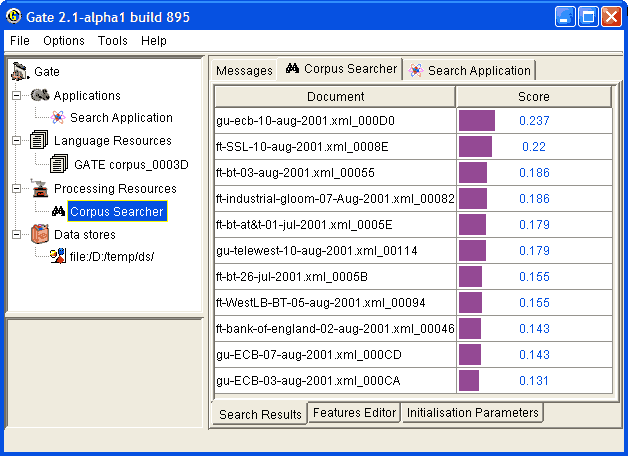
\includegraphics[scale=0.5]{ir1.png}
\end{center}
\caption{Documents with scores, returned from a search over a corpus}
\label{fig:ir1}
\end{figure}
%


\begin{table}
\begin{center}
\begin{tabular}{|c|c|c|c|c|c|}
\hline
& $term_1$ & $term_2$ & ... & ... & $term_k$\\
\hline
$doc_1$ & $w_{1,1}$ & $w_{1,2}$ & ... & ... & $w_{1,k}$\\
\hline
$doc_2$ & $w_{2,1}$ & $w_{2,1}$ & ... & ... & $w_{2,k}$\\
\hline
... & ... & ... & ... & ... & ... \\
\hline
... & ... & ... & ... & ... & ... \\
\hline
$doc_n$ & $w{_n,1}$ & $w_{n,2}$ & ... & ... & $w_{n,k}$\\
\hline
\end{tabular}
\caption{An information retrieval document-term matrix}
\label{table:matrix}
\end{center}
\end{table}



Information Retrieval systems usually perform some preprocessing one the input
corpus in order to create the document-term matrix for the corpus. A
document-term matrix is usually presented as in Table~\ref{table:matrix},
where $doc_i$ is a document from the corpus, $term_j$ is a word that is
considered as important and representative for the document and $wi,j$ is the
weight assigned to the term in the document. There are many ways to define the
term weight functions, but most often it depends on the term frequency in the
document and in the whole corpus (i.e. the local and the global
frequency). Note that the machine learning plugin described in
\Chapthing~\ref{chap:ml} can produce such document-term matrix (for detailed
description of the matrix produced, see Section \ref{sec:ml:feature}).

Note that not all of the words appearing in the document are
considered terms. There are many words (called `stop-words') which are
ignored, since they are observed too often and are not representative
enough. Such words are articles, conjunctions, etc. During the
preprocessing phase which identifies such words, usually a form of
stemming is performed in order to minimize the number of terms and to
improve the retrieval recall. Various forms of the same word
(e.g. `play', `playing' and `played') are considered identical and
multiple occurrences of the same term (probably `play') will be
observed.

It is recommended that the user reads the relevant Information
Retrieval literature for a detailed explanation of stop words,
stemming and term weighting.

IR systems, in a way similar to IE systems, are evaluated with the
help of the precision and recall measures (see Section
\ref{sec:eval:metrics} for more details).


%%%%%%%%%%%%%%%%%%%%%%%%%%%%%%%%%%%%%%%%%%%%%%%%%%%%%%%%%%%%%%%%%%%%%%%%%%%%%
\subsect{Using the IR Functionality in GATE}
%%%%%%%%%%%%%%%%%%%%%%%%%%%%%%%%%%%%%%%%%%%%%%%%%%%%%%%%%%%%%%%%%%%%%%%%%%%%%

In order to run queries against a corpus, the latter should be
`indexed'. The indexing process first processes the documents in order
to identify the terms and their weights (stemming is performed too)
and then creates the proper structures on the local file system. These
file structures contain indexes that will be used by Lucene (the
underlying IR engine) for the retrieval.

Once the corpus is indexed, queries may be run against
it. Subsequently the index may be removed and then the structures on
the local file system are removed too. Once the index is removed,
queries cannot be run against the corpus.

\subsubsect{Indexing the Corpus}

In order to index a corpus, the latter should be stored in a serial
datastore. In other words, the IR functionality is unavailable for
corpora that are transient or stored in a RDBMS datastores (though
support for the latter may be added in the future).

To index the corpus, follow these steps:

\begin{itemize}
%
\item
Select the corpus from the resource tree (top-left pane) and from the
context menu (right button click) choose `Index Corpus'. A dialogue
appears that allows you to specify the index properties.
%
\item
In the index properties dialogue, specify the underlying IR system to
be used (only Lucene is supported at present), the directory that will
contain the index structures, and the set of properties that will be
indexed such as document features, content, etc (the same properties
will be indexed for each document in the corpus).
%
\item
Once the corpus in indexed, you may start running queries against
it. Note that the directory specified  for the index data should exist
and be empty. Otherwise an error will occur during the index creation.
%
\end{itemize}

%
\begin{figure}[htbp]
\begin{center}
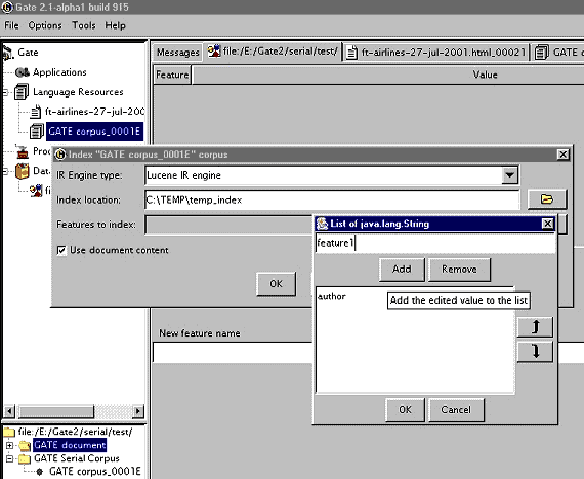
\includegraphics[scale=0.5]{ir2.png}
\end{center}
\caption{Indexing a corpus by specifying the index location and
indexed features (and content)}
\label{fig:ir2}
\end{figure}
%

\subsubsect{Querying the Corpus}


To query the corpus, follow these steps:

\begin{itemize}
%
\item
Create a SearchPR processing resource. All the parameters of SearchPR
are runtime so they are set later.
%
\item
Create a ``pipeline'' application ({\em not} a ``corpus pipeline'') containing
the SearchPR.
%
\item
Set the following SearchPR parameters:
 \begin{itemize}
 %
 \item
 The corpus that will be queried.
  %
 \item
 The query that will be executed.
  %
 \item
 The maximum number of documents returned.
 \end{itemize}

A query looks like the following:

\begin{verbatim}
{+/-}field1:term1 {+/-}field2:term2 ? {+/-}fieldN:termN
\end{verbatim}
where \texttt{field} is the name of a index field, such as the one specified at
index creation (the document content field is body) and term is a term
that should appear in the field.

For example the query:
\begin{verbatim}
+body:government +author:CNN
\end{verbatim}
will inspect the document content for the term `government' (together
with variations such as `governments' etc.) and the index field named
`author' for the term `CNN'. The `author' field is specified at index
creation time, and is either a document feature or another document
property.

%
\item
After the SearchPR is initialized, running the application executes
the specified query over the specified corpus.

%
\item
Finally, the results are displayed (see fig.1) after a double-click on
the SearchPR processing resource.
%
\end{itemize}

\subsubsect{Removing the Index}

An index for a corpus may be removed at any time from the `Remove
Index' option of the context menu for the indexed corpus (right button
click).


%%%%%%%%%%%%%%%%%%%%%%%%%%%%%%%%%%%%%%%%%%%%%%%%%%%%%%%%%%%%%%%%%%%%%%%%%%%%%
\subsect{Using the IR API}
%%%%%%%%%%%%%%%%%%%%%%%%%%%%%%%%%%%%%%%%%%%%%%%%%%%%%%%%%%%%%%%%%%%%%%%%%%%%%

The IR API within GATE Embedded makes it possible for corpora to be
indexed, queried and results returned from any Java application,
without using GATE Developer. The following sample indexes a corpus,
runs a query against it and then removes the index.

\begin{lstlisting}

// open a serial datastore
SerialDataStore sds =
Factory.openDataStore("gate.persist.SerialDataStore",
"/tmp/datastore1");
sds.open();

//set an AUTHOR feature for the test document
Document doc0 = Factory.newDocument(new URL("/tmp/documents/doc0.html"));
doc0.getFeatures().put("author","John Smith");

Corpus corp0 = Factory.newCorpus("TestCorpus");
corp0.add(doc0);

//store the corpus in the serial datastore
Corpus serialCorpus = (Corpus) sds.adopt(corp0,null);
sds.sync(serialCorpus);

//index the corpus -  the content and the AUTHOR feature

IndexedCorpus indexedCorpus = (IndexedCorpus) serialCorpus;

DefaultIndexDefinition did = new DefaultIndexDefinition();
did.setIrEngineClassName(
  gate.creole.ir.lucene.LuceneIREngine.class.getName());
did.setIndexLocation("/tmp/index1");
did.addIndexField(new IndexField("content",
  new DocumentContentReader(), false));
did.addIndexField(new IndexField("author", null, false));
indexedCorpus.setIndexDefinition(did);

indexedCorpus.getIndexManager().createIndex();
//the corpus is now indexed

//search the corpus
Search search = new LuceneSearch();
search.setCorpus(ic);

QueryResultList res = search.search("+content:government +author:John");

//get the results
Iterator it = res.getQueryResults();
while (it.hasNext()) {
QueryResult qr = (QueryResult) it.next();
System.out.println("DOCUMENT_ID=" + qr.getDocumentID()
  + ",   score=" + qr.getScore());
}

\end{lstlisting}

%%%%%%%%%%%%%%%%%%%%%%%%%%%%%%%%%%%%%%%%%%%%%%%%%%%%%%%%
\sect[sec:misc-creole:crawler]{Websphinx Web Crawler}
%%%%%%%%%%%%%%%%%%%%%%%%%%%%%%%%%%%%%%%%%%%%%%%%%%%%%%%%%
The `Web\_Crawler\_Websphinx' plugin enables GATE to build a corpus from a web
crawl.  It is based on
\htlink{http://www.cs.cmu.edu/~rcm/websphinx/}{Websphinx}, a JAVA-based,
customizable, multi-threaded web crawler.


\textbf{Note:} if you are using this plugin via an IDE, you may need to make
sure that the websphinx.jar file is on the IDE's classpath, or add it to the
IDE's lib directory.


The basic idea is to specify a source URL (or set of documents created from web
URLs) and a depth and maximum number of documents to build the initial corpus
upon which further processing could be done.  The PR itself provides a number of
other parameters to regulate the crawl.


This PR now uses the HTTP \texttt{Content-Type} headers to determine each web
page's encoding and MIME type before creating a GATE Document from it.  It also
adds to each document a \emph{Date} feature (with a \texttt{java.util.Date}
value) based on the HTTP \texttt{Last-Modified} header (if available) or the
current timestamp, an \emph{originalMimeType} feature taken from the
\texttt{Content-Type} header, and an \emph{originalLength} feature indicating
the size in bytes of the downloaded document.
%%%%%%%%%%%%%%%%%%%%%%%%%%%%%%%%%%%%%%%%%%%%%%%%%%%%%%%%%%%%%%%%%%%%%%%%%%%%%
\subsect{Using the Crawler PR}
%%%%%%%%%%%%%%%%%%%%%%%%%%%%%%%%%%%%%%%%%%%%%%%%%%%%%%%%%%%%%%%%%%%%%%%%%%%%%
In order to use the processing resource you need to load the plugin using the
plugin manager, create an instance of the crawl PR from the list of processing
resources, and create a corpus in which to store crawled documents. In order to
use the crawler, create a simple pipeline (\textbf{not} a corpus pipeline) and
add the crawl PR to the pipeline.

Once the crawl PR is created there will be a number of parameters that can be
set based on the PR required (see also Figure~\ref{fig:crawler-parameters}).
%
\begin{figure}[htb]
  \begin{center}
    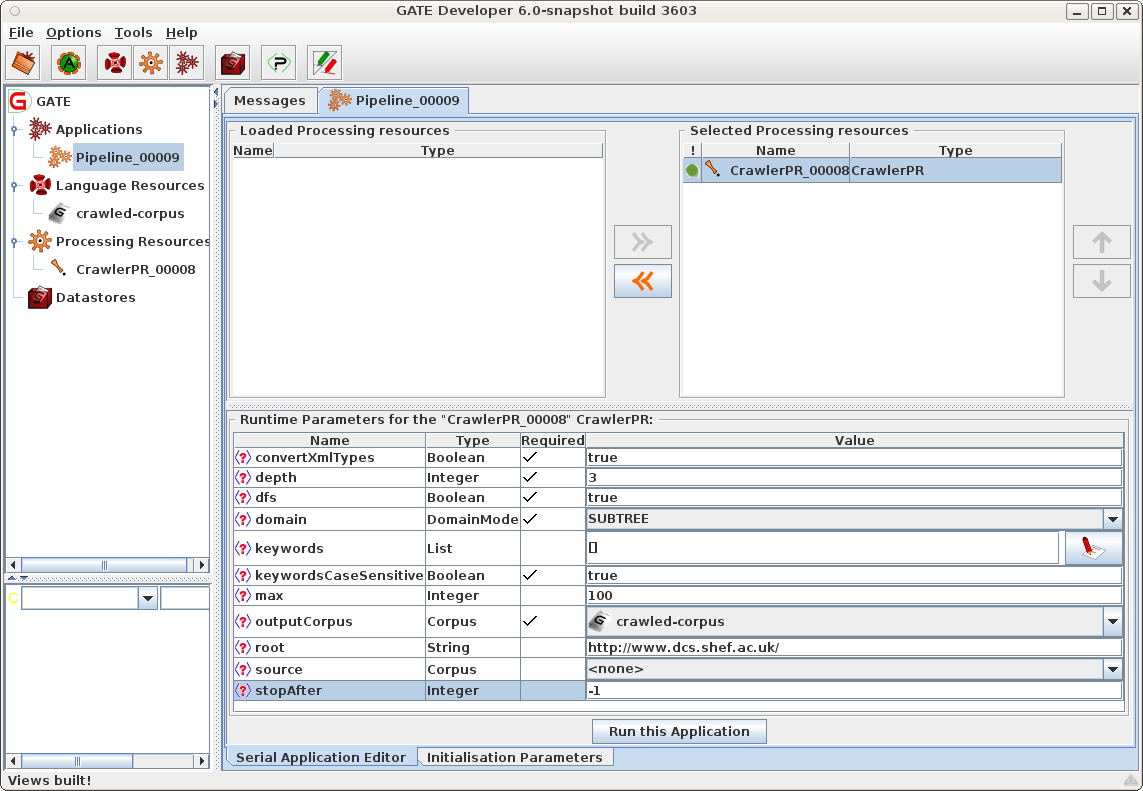
\includegraphics[width=\textwidth]{crawler-parameters.png}
  \end{center}
  \caption{Crawler parameters}
  \label{fig:crawler-parameters}
\end{figure}
% 
\begin{description}
\item[depth] The depth (integer) to which the crawl should proceed.
\item[dfs] A boolean:
  \begin{description}
  \item[true] the crawler visits links with a depth-first strategy;
  \item[false] the crawler visits links with a breadth-first strategy;
  \end{description}
\item[domain] An \texttt{enum} value, presented as a pull-down list in the GUI:
  \begin{description}
  \item[SUBTREE] The crawler visits only the descendents of the pages
    specified as the roots for the crawl.
  \item[WEB] The crawler can visit any pages on the web.
  \item[SERVER] The crawler can visit only pages that are present on the
    server where the root pages are located.
  \end{description}
\item[max] The maximum number (integer) of pages to be kept: the crawler will
  stop when it has stored this number of documents in the output corpus.  Use
  $-1$ to ignore this limit.
\item[maxPageSize] The maximum page size in kB; pages over this limit will be
  ignored---even as roots of the crawl---and their links will not be crawled.
  If your crawl does not add any documents (even the seeds) to the output
  corpus, try increasing this value.  (A 0 or negative value here means ``no
  limit''.)
\item[stopAfter] The maximum number (integer) of pages to be fetched: the
  crawler will stop when it has visited this number of pages.  Use $-1$ to
  ignore this limit.  If $\mathit{max} > \mathit{stopAfter} > 0$ then the
  crawl will store at most \emph{stopAfter} (not \emph{max}) documents.
\item[root] A string containing one URL to start the crawl.
\item[source] A corpus that contains the documents whose
  \texttt{gate.sourceURL} features will be used to start the crawl.  If you
  use both \emph{root} and \emph{source} parameters, both the \emph{root}
  value and the URLs collected from the \emph{source} documents will seed the
  crawl.
\item[outputCorpus] The corpus in which the fetched documents will be stored.
\item[keywords] A \texttt{List<String>} for matching against crawled
  documents.  If this list is empty or null, all documents fetched will be
  kept.  Otherwise, only documents that contain one of these strings will be
  stored in the output corpus.  (Documents that are fetched but not kept are
  still scanned for further links.)
\item[keywordsCaseSensitive] This boolean determines whether keyword matching
  is case-sensitive or not.
\item[convertXmlTypes] GATE's \texttt{XmlDocumentFormat} only accepts certain
  MIME types.  If this parameter is true, the crawl PR converts other XML
  types (such as \texttt{application/atom+xml.xml}) to \texttt{text/xml}
  before trying to instantiate the GATE document (this allows GATE to handle
  RSS feeds, for example).
\item[userAgent] If this parameter is blank, the crawler will use the default
  Websphinx user-agent header.  Set this parameter to spoof the header.
\end{description}


Once the parameters are set, the crawl can be run and the documents fetched (and
matched to the keywords, if that list is in use) are added to the specified
corpus.  Documents that are fetched but not matched are discarded after scanning
them for further links.  
% Figure \ref{fig:crawler-corpus} shows the crawled pages
% added to the corpus.
% %
% \begin{figure}[htb]
% \begin{center}
% 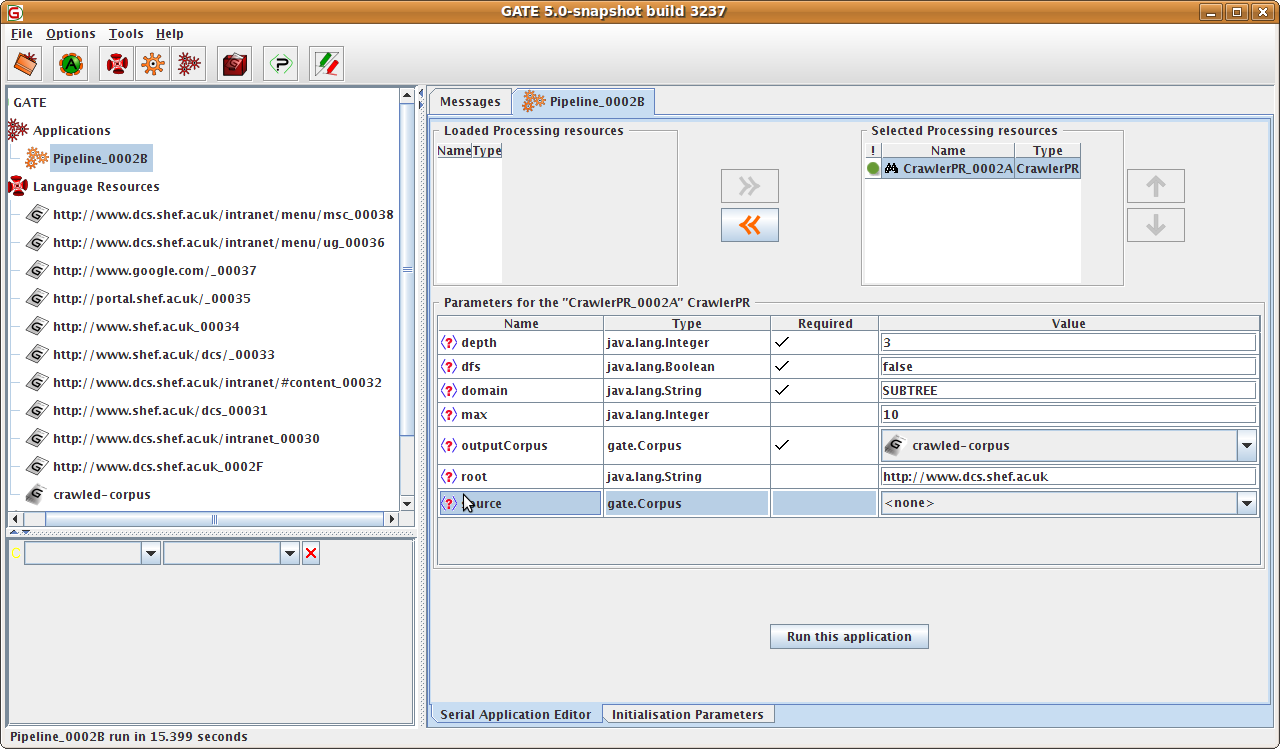
\includegraphics[width=\textwidth]{crawler-corpus.png}
% \end{center}
% \caption{Crawled pages added to the corpus}
% \label{fig:crawler-corpus}
% \end{figure}


\textbf{Note} that you must use a simple Pipeline, and not a Corpus Pipeline. In
order to process the corpus of crawled documents, you need to build a separate
Corpus Pipeline and run it after crawling.  You could combine the two functions
by carefully developing a Scriptable Controller (see
section~\ref{sec:api:groovy:controller} for details).
%%%%%%%%%%%%%%%%%%%%%%%%%%%%%%%%%%%%%%%%%%%%%%%%%%%%%%%%%%%%%%%%%%%%%%%%%%%%%
\subsect[sec:misc-creole:proxy]{Proxy configuration}
%%%%%%%%%%%%%%%%%%%%%%%%%%%%%%%%%%%%%%%%%%%%%%%%%%%%%%%%%%%%%%%%%%%%%%%%%%%%%
The underlying WebSPHINX crawler uses Java's \emph{URLConnection} class, which
respects the JVM's proxy configuration (if it is set).  To configure a proxy for
GATE Developer, edit or create the file \texttt{build.properties} and add the
following lines (the first line is required, and the rest should be changed as
necessary for your configuration):
\begin{verbatim}
run.java.net.useSystemProxies=true
http.proxyHost=proxy.example.com
http.proxyPort=8080
http.nonProxyHosts=*.example.com
\end{verbatim}
Save the file and restart GATE Developer and it should start using your
configured proxy settings.  The proxy server, port, and exceptions can also be
set using the Java control panel, but GATE will use them only if
\texttt{run.java.net.useSystemProxies=true} is set in the
\texttt{build.properties} file.  Consult the Oracle \emph{Java Networking and
  Proxies} documentation\footnote{see
  \url{http://docs.oracle.com/javase/6/docs/technotes/guides/net/proxies.html}}
for further details of proxy configuration in Java, and see 
section~\ref{sec:gettingstarted:sysprop}.

With effect from build 4723 (14 November 2013), the proxy and other options can
be configured in the \texttt{gate.l4j.ini} file on all platforms, as explained
in Section~\ref{sec:gettingstarted:launchconfig}.
%%%%%%%%%%%%%%%%%%%%%%%%%%%%%%%%%%%%%%%%%%%%%%%%%%%%%%%%%%%%%%%%%%%%%%%%%%%%%
\sect[sec:misc-creole:wn]{WordNet in GATE}
%%%%%%%%%%%%%%%%%%%%%%%%%%%%%%%%%%%%%%%%%%%%%%%%%%%%%%%%%%%%%%%%%%%%%%%%%%%%%
%
\begin{figure}[htb]
\begin{center}
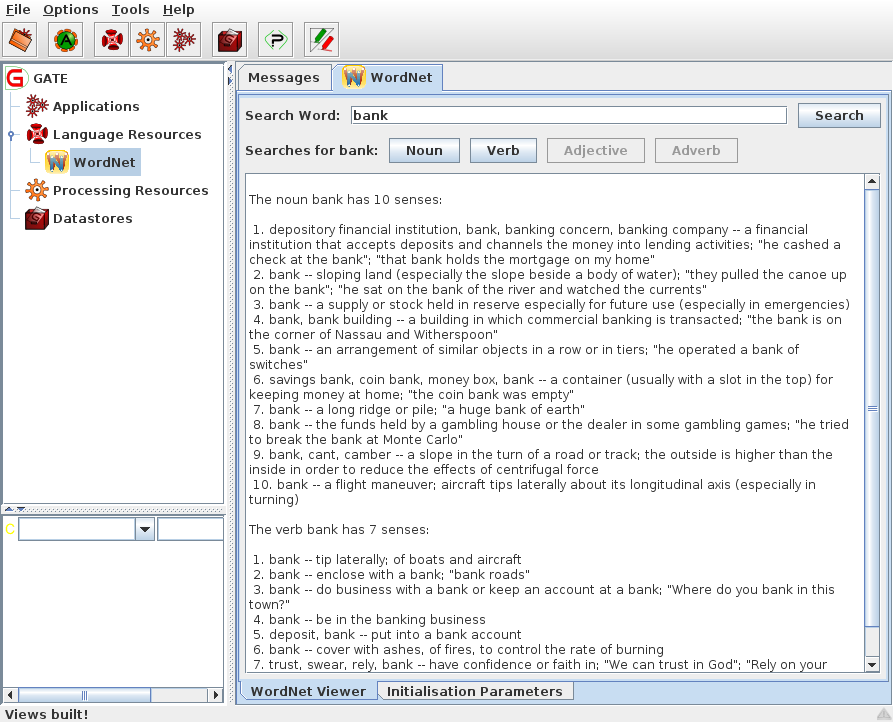
\includegraphics[scale=0.5]{wordnet1.png}
\end{center}
\caption{WordNet in GATE -- results for `bank'}
\label{fig:wordnet1}
\end{figure}
%
%
\begin{figure}
\begin{center}
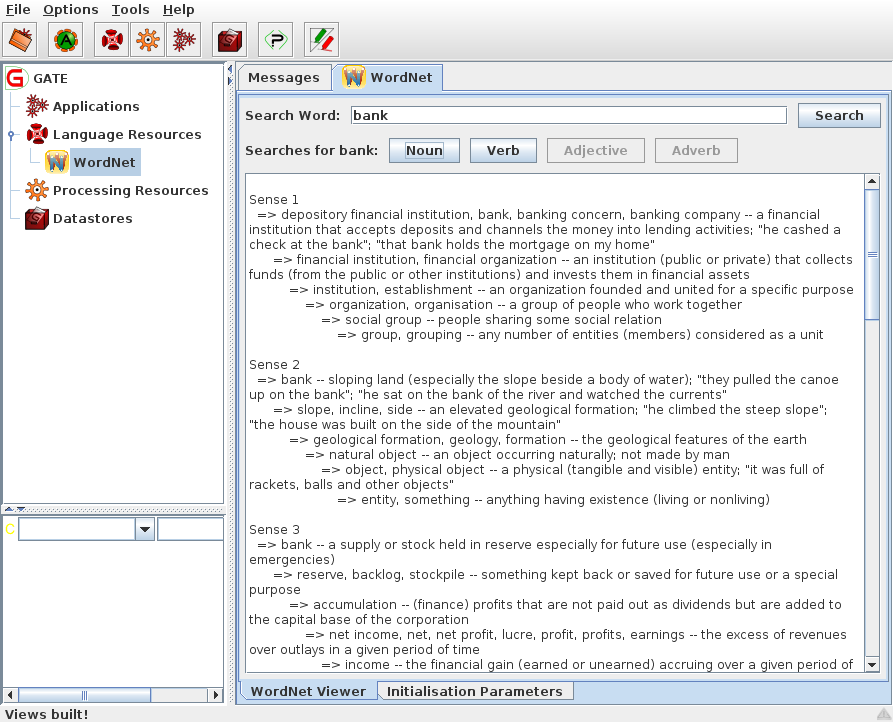
\includegraphics[scale=0.5]{wordnet3.png}
\end{center}
\caption{WordNet in GATE}
\label{fig:wordnet3}
\end{figure}
%
GATE currently supports versions 1.6 and newer of WordNet, so in order to use
WordNet in GATE, you must first install a compatible version of WordNet on your
computer. WordNet is available at
\htlinkplain{http://wordnet.princeton.edu/}. The next step is to
configure GATE to work with your local WordNet installation. Since
GATE relies on the Java WordNet Library (JWNL) for WordNet access,
this step consists of providing one special xml file that is used
internally by JWNL. This file describes the location of your local
copy of the WordNet index files. An example of this wn-config.xml
file is shown below:

\begin{small}
\begin{verbatim}

<?xml version="1.0" encoding="UTF-8"?>
<jwnl_properties language="en">
  <version publisher="Princeton" number="3.0" language="en"/>
  <dictionary class="net.didion.jwnl.dictionary.FileBackedDictionary">
    <param name="morphological_processor"
       value="net.didion.jwnl.dictionary.morph.DefaultMorphologicalProcessor">
    <param name="operations">
       <param value=
          "net.didion.jwnl.dictionary.morph.LookupExceptionsOperation"/>
       <param value="net.didion.jwnl.dictionary.morph.DetachSuffixesOperation">
          <param name="noun" 
             value="|s=|ses=s|xes=x|zes=z|ches=ch|shes=sh|men=man|ies=y|"/>
          <param name="verb" 
             value="|s=|ies=y|es=e|es=|ed=e|ed=|ing=e|ing=|"/>
          <param name="adjective" 
             value="|er=|est=|er=e|est=e|"/>
          <param name="operations">
             <param 
                value="net.didion.jwnl.dictionary.morph.LookupIndexWordOperation"/>
             <param 
                value="net.didion.jwnl.dictionary.morph.LookupExceptionsOperation"/>
          </param>
       </param>
       <param value="net.didion.jwnl.dictionary.morph.TokenizerOperation">
          <param name="delimiters">
             <param value=" "/>
             <param value="-"/>
          </param>
          <param name="token_operations">
             <param 
                value="net.didion.jwnl.dictionary.morph.LookupIndexWordOperation"/>
             <param 
                value="net.didion.jwnl.dictionary.morph.LookupExceptionsOperation"/>
             <param 
                value="net.didion.jwnl.dictionary.morph.DetachSuffixesOperation">
                <param name="noun" 
                   value="|s=|ses=s|xes=x|zes=z|ches=ch|shes=sh|men=man|ies=y|"/>
                <param name="verb" 
                   value="|s=|ies=y|es=e|es=|ed=e|ed=|ing=e|ing=|"/>
                <param name="adjective" value="|er=|est=|er=e|est=e|"/>
                <param name="operations">
                   <param value=
                      "net.didion.jwnl.dictionary.morph.LookupIndexWordOperation"/>
                   <param value=
                      "net.didion.jwnl.dictionary.morph.LookupExceptionsOperation"/>
                </param>
             </param>
          </param>
       </param>
    </param>
  </param>
      <param name="dictionary_element_factory" value=
         "net.didion.jwnl.princeton.data.PrincetonWN17FileDictionaryElementFactory"/>
      <param name="file_manager" value=
         "net.didion.jwnl.dictionary.file_manager.FileManagerImpl">
         <param name="file_type" value=
            "net.didion.jwnl.princeton.file.PrincetonRandomAccessDictionaryFile"/>
         <param name="dictionary_path" value="/home/mark/WordNet-3.0/dict/"/>
      </param>
   </dictionary>
   <resource class="PrincetonResource"/>
</jwnl_properties>
\end{verbatim}
\end{small}

There are three things in this file which you need to configure based upon the
version of WordNet you wish to use.  Firstly change the \verb|number| attribute
of the \verb|version| element to match the version of WordNet you are using.
Then edit the value of the \verb|dictionary_path| parameter to point to your
local installation of WordNet (this is \verb!/usr/share/wordnet/! if you have
installed the Ubuntu or Debian \texttt{wordnet-base} package.)


Finally, if you want to use version 1.6 of WordNet then you also need to alter
the \verb|dictionary_element_factory| to use
\verb|net.didion.jwnl.princeton.data.PrincetonWN16FileDictionaryElementFactory|. For
full details of the format of the configuration file see the JWNL documentation
at~\url{http://sourceforge.net/projects/jwordnet}.

After configuring GATE to use WordNet, you can start using the
built-in WordNet browser or API. In GATE Developer, load the WordNet
plugin via the Plugin Management Console. Then load WordNet by selecting it from
the set of available language resources. Set the value of the
parameter to the path of the xml properties file which describes the
WordNet location (wn-config).

Once WordNet is loaded in GATE Developer, the well-known interface of
WordNet will appear. You can search Word Net by typing a word in the
box next to to the label `SearchWord'' and then pressing
`Search'. All the senses of the word will be displayed in the window
below.  Buttons for the possible parts of speech for this word will
also be activated at this point.  For instance, for the word `play',
the buttons `Noun', `Verb' and `Adjective' are activated.
Pressing one of these buttons will activate a menu with hyponyms,
hypernyms, meronyms for nouns or verb groups, and cause for verbs,
etc. Selecting an item from the menu will display the results in the
window below.

To upgrade any existing GATE applications to use this improved WordNet plugin simply replace your
existing configuration file with the example above and configure for WordNet 1.6. This will then
give results identical to the previous version -- unfortunately it was not possible to provide
a transparent upgrade procedure.

More information about WordNet can be found
at~\url{http://wordnet.princeton.edu/}

More information about the JWNL library can be found
at~\url{http://sourceforge.net/projects/jwordnet}

An example of using the WordNet API in GATE is available on the GATE examples
page at~\url{http://gate.ac.uk/wiki/code-repository/index.html}.

%%%%%%%%%%%%%%%%%%%%%%%%%%%%%%%%%%%%%%%%%%%%%%%%%%%%%%%%%%%%%%%%%%%%%%%%%%%%%
\subsect{The WordNet API}
%%%%%%%%%%%%%%%%%%%%%%%%%%%%%%%%%%%%%%%%%%%%%%%%%%%%%%%%%%%%%%%%%%%%%%%%%%%%%

GATE Embedded offers a set of classes that can be used to access the
WordNet Lexical Database. The implementation of the GATE API
for WordNet is based on Java WordNet Library (JWNL). There are just a
few basic classes, as shown in Figure
\ref{fig:wordnet4}. Details about the properties and methods of the
interfaces/classes comprising the API can be obtained from the
JavaDoc. Below is a brief overview of the interfaces:
\begin{itemize}
\item \textbf{WordNet}: the main WordNet class. Provides methods for getting the
synsets of a lemma, for accessing the unique beginners, etc.

\item \textbf{Word}: offers access to the word's lemma and senses

\item \textbf{WordSense}: gives access to the synset, the word, POS
and lexical relations.

\item \textbf{Synset}: gives access to the word senses (synonyms) in
the synset, the semantic relations, POS etc.

\item \textbf{Verb}: gives access to the verb frames (not working
properly at present)

\item \textbf{Adjective}: gives access to the adj. position
(attributive, predicative, etc.).

\item \textbf{Relation}: abstract relation such as type, symbol,
inverse relation, set of POS tags, etc. to which it is applicable.

\item \textbf{LexicalRelation}

\item \textbf{SemanticRelation}

\item \textbf{VerbFrame}
\end{itemize}

\begin{figure}[!htb]
\begin{center}
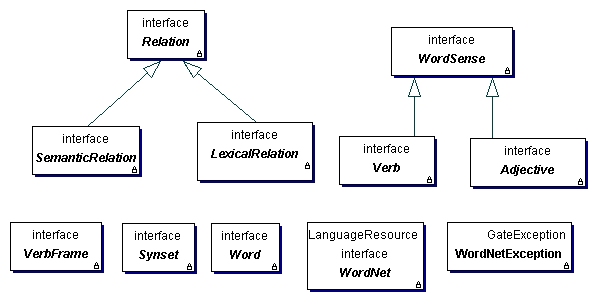
\includegraphics[scale=1]{wordnet4.png}
\caption{The Wordnet API}
\label{fig:wordnet4}
\end{center}
\end{figure}





%%%%%%%%%%%%%%%%%%%%%%%%%%%%%%%%%%%%%%%%%%%%%%%%%%%%%%%%%%%%%%%%%%%%%%%%%%%%%
%\sect[sect:ml]{Machine Learning in GATE}
%%%%%%%%%%%%%%%%%%%%%%%%%%%%%%%%%%%%%%%%%%%%%%%%%%%%%%%%%%%%%%%%%%%%%%%%%%%%%

%\textbf{Note:} A brand new machine learning layer specifically targetted at NLP
%tasks including text classification, chunk learning (e.g. for named entity
%recognition) and relation learning has been added to GATE. See
%chapter~\ref{chapt:mlapi} for more details.

%This section presents machine learning PRs available in
%GATE. Currently, two PRs are available:
%
%\begin{itemize}
%
%\item{The \textbf{Batch Learning PR} (in the \textbf{learning} plugin) is
%GATE's most comprehensive and developed machine learning offering. It is
%specifically targetted at NLP tasks including text classification, chunk
%learning (e.g. for named entity recognition) and relation learning. It
%integrates LibSVM for improved speed. It also offers a Weka interface. It is
%introduced briefly in section~\ref{sect:learning-pr} and documented more fully
%in \Chapthing~\ref{chapt:mlapi}. \Chapthing~\ref{chapt:mlapi} also provides a
%short introduction to machine learning, in which concepts are defined.}
%
%\item{The \textbf{Machine Learning PR} (in the \textbf{Machine\_Learning}
%plugin) is GATE's older machine learning offering. It offers wrappers for
%Maxent, Weka and SVM Light. It is documented in
%section~\ref{sect:machine-learning-pr}.}
%
%\end{itemize}
%
%\subsect[sect:learning-pr]{Batch Learning PR}
%
%The Batch Learning PR/API provides a new machine learning layer in
%GATE designed particularly for NLP learning. It can be used for text
%classification, chunk recognition, and relation extraction; this
%covers much of the functionality required in NLP. These different
%types of task are described in \chapthing~\ref{chapt:mlapi}.
%
%The PR/API implements suitable feature representations for the three
%types of NLP learning. It provides implementations of widely used ML
%algorithms such as SVM, KNN, Naive Bayes, and the decision tree
%algorithm C4.5. Furthermore, it can process a GATE corpus into feature
%sets suitable for use with other machine learning algorithms outside
%of GATE.
%
%The PR, particularly the SVM functionality, has been developed through
%use over several years and has been used to produce state of the art
%results in for example the NTCIR-6 Patent Retrieval
%Task \cite{Yaoyong07b}. \Chapthing~\ref{chapt:mlapi} is devoted to
%fully documenting the Batch Learning PR/API.

%%%%%%%%%%%%%%%%%%%%%%%%%%%%%%%%%%%%%%%%%%
% \sect[sec:misc-creole:probability]{Probability Finder}
% 
% The probability finder PR is used to obtain the probabilities for the occurrences of
% each of the named entities found in a corpus.
% 
% The following describes the basic steps to use it
% \begin{itemize}
% 
% \item Build the corpus either manually adding documents or by querying Google or
% crawling the WWW
% 
% \item Once the corpus is built, load ANNIE
% 
% \item Perform any processing required to find the Named Entities, using any JAPE
% Transducers, etc.
% 
% \item Load the ProbabilityPR via the Manage Plugins menu
% 
% \item Create a new pipeline or add the Probability PR to the existing pipeline.
% 
% \item In the runtime parameters, you will see the following options:
%     \begin{itemize}
%     \item the Entity Type to be used, e.g. Person, Location, Organization.
%  (Note that you can use only entities in the Default Annotation Set, and that you can only use one entity type at a time)
%     \item the processed corpus to be used.
%     \end{itemize}
% 
% \item Once run, the output in the messages tab will correspond to the basic
% probabilistic outcomes of occurrence for each entity. Please note that there is
% no co-reference resolution done.
% \end{itemize}
% 
%%%%%%%%%%%%%%%%%%%%%%%%%%%%%%%%%%%%%%%%%%%%%%%%%%%%%%%%%%%%%%%%%%%%%%%%%%%%%

%%%%%%%%%%%%%%%%%%%%%%%%%%%%%%%%%%%%%%%%%%%%%%%%%%%%%%%%%%%%%%%%%%%%%%%%%%%%%
\sect[sec:misc-creole:kea]{Kea - Automatic Keyphrase Detection}
%%%%%%%%%%%%%%%%%%%%%%%%%%%%%%%%%%%%%%%%%%%%%%%%%%%%%%%%%%%%%%%%%%%%%%%%%%%%%

Kea is a tool for automatic detection of key phrases developed at
the University of Waikato in New Zealand. The home page of the project can be
found at \url{http://www.nzdl.org/Kea/}.

This user guide section only deals with the aspects relating to the integration
of Kea in GATE. For the inner workings of Kea, please visit the Kea web site
and/or contact its authors.

In order to use Kea in GATE Developer, the `Keyphrase\_Extraction\_Algorithm'
plugin needs to be loaded using the plugins management console. After doing that,
two new resource types are available for creation: the `KEA Keyphrase
Extractor' (a processing resource) and the `KEA Corpus Importer' (a visual
resource associated with the PR).

%%%%%%%%%%%%%%%%%%%%%%%%%%%%%%%%%%%%%%%%%%%%%%%%%%%%%%%%%%%%%%%%%%%%%%%%%%%%%
\subsect{Using the `KEA Keyphrase Extractor' PR}
%%%%%%%%%%%%%%%%%%%%%%%%%%%%%%%%%%%%%%%%%%%%%%%%%%%%%%%%%%%%%%%%%%%%%%%%%%%%%

Kea is based on machine learning and it needs to be trained before it can be
used to extract keyphrases. In order to do this, a corpus is required where the
documents are annotated with keyphrases. Corpora in the Kea format (where the
text and keyphrases are in separate files with the same name but different
extensions) can be imported into GATE using the `KEA Corpus Importer' tool.
The usage of this tool is presented in a subsection below.

Once an annotated corpus is obtained, the `KEA Keyphrase Extractor' PR can be
used to build a model:
\begin{enumerate}
\item load a `KEA Keyphrase Extractor'
\item create a new `Corpus Pipeline' controller.
\item set the corpus for the controller
\item set the `trainingMode' parameter for the PR to `true'
\item run the application.
\end{enumerate}

After these steps, the Kea PR contains a trained model. This can be used
immediately by switching the `trainingMode' parameter to `false' and running the
PR over the documents that need to be annotated with keyphrases. Another
possibility is to save the model for later use, by right-clicking on the PR name
in the right hand side tree and choosing the `Save model' option.

When a previously built model is available, the training procedure does not
need to be repeated, the existing model can be loaded in memory by selecting
the `Load model' option in the PR's context menu.
\begin{figure}
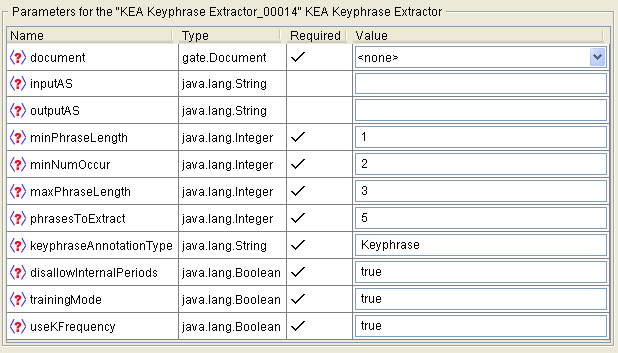
\includegraphics[scale=0.75]{keaParams.png}
\caption{Parameters used by the Kea PR}
\label{fig:keaParams}
\end{figure}

The Kea PR uses several parameters as seen in Figure~\ref{fig:keaParams}:
\begin{description}
\item[document] The document to be processed.
\item[inputAS] The input annotation set. This parameter is only relevant when
the PR is running in training mode and it specifies the annotation set containing
the keyphrase annotations.
\item[outputAS] The output annotation set. This parameter is only relevant when
the PR is running in application mode (i.e. when the `trainingMode' parameter is
set to false) and it specifies the annotation set where the generated keyphrase
annotations will be saved.
\item[minPhraseLength] the minimum length (in number of words) for a keyphrase.
\item[minNumOccur] the minimum number of occurrences of a phrase for it to be a
keyphrase.
\item[maxPhraseLength] the maximum length of a keyphrase.
\item[phrasesToExtract] how many different keyphrases should be generated.
\item[keyphraseAnnotationType] the type of annotations used for keyphrases.
\item[dissallowInternalPeriods] should internal periods be disallowed.
\item[trainingMode] if `true' the PR is running in training mode; otherwise it
is running in application mode.
\item[useKFrequency] should the K-frequency be used.
\end{description}


%%%%%%%%%%%%%%%%%%%%%%%%%%%%%%%%%%%%%%%%%%%%%%%%%%%%%%%%%%%%%%%%%%%%%%%%%%%%%
\subsect{Using Kea Corpora}
%%%%%%%%%%%%%%%%%%%%%%%%%%%%%%%%%%%%%%%%%%%%%%%%%%%%%%%%%%%%%%%%%%%%%%%%%%%%%

The authors of Kea provide on the project web page a few manually annotated
corpora that can be used for training Kea. In order to do this from within GATE,
these corpora need to be converted to the format used in GATE (i.e. GATE
documents with annotations). This is possible using the `KEA Corpus Importer'
tool which is available as a visual resource associated with the Kea PR. The
importer tool can be made visible by double-clicking on the Kea PR's name in the
resources tree and then selecting the `KEA Corpus Importer' tab, see
Figure~\ref{fig:keaImporter}.

\begin{figure}
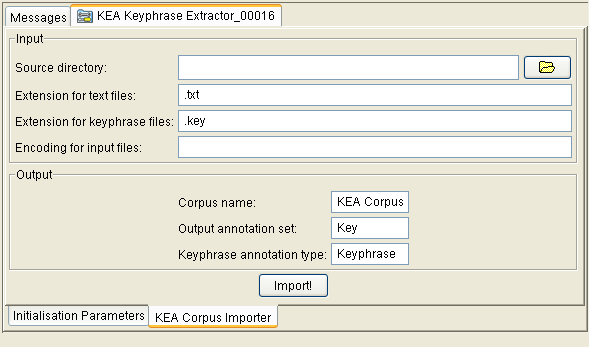
\includegraphics[scale=0.75]{keaCorpusImporter.png}
\caption{Options for the `KEA Corpus Importer'}
\label{fig:keaImporter}
\end{figure}

The tool will read files from a given directory, converting the text ones into
GATE documents and the ones containing keyphrases into annotations over the
documents.

The user needs to specify a few values:
\begin{description}
\item[Source Directory] the directory containing the text and key files. This
can be typed in or selected by pressing the folder button next to the text
field.
\item[Extension for text files] the extension used for text fields (by default
.txt).
\item[Extension for keyphrase files] the extension for the files listing
keyphrases.
\item[Encoding for input files] the encoding to be used when reading the files.
\item[Corpus name] the name for the GATE corpus that will be created.
\item[Output annotation set] the name for the annotation set that will contain
the keyphrases read from the input files.
\item[Keyphrase annotation type] the type for the generated annotations.
\end{description}


%%%%%%%%%%%%%%%%%%%%%%%%%%%%%%%%%%%%%%%%%%%%%%%%%%%%%%%%%%%%%%%%%%%%%%%%%%%%%
\sect[sec:misc-creole:merging]{Annotation Merging Plugin}
%%%%%%%%%%%%%%%%%%%%%%%%%%%%%%%%%%%%%%%%%%%%%%%%%%%%%%%%%%%%%%%%%%%%%%%%%%%%%


If we have annotations about the same subject on the same document from
different annotators, we may need to merge the annotations.

This plugin implements two approaches for annotation merging.

{\em MajorityVoting} takes a parameter {\em numMinK} and selects the
annotation on which at least {\em numMinK} annotators agree. If two or more
merged annotations have the same span, then the annotation with the most
supporters is kept and other annotations with the same span are discarded.

{\em MergingByAnnotatorNum} selects one annotation from those annotations with
the same span, which the majority of the annotators support. Note that if one
annotator did not create the annotation with the particular span, we count it
as one non-support of the annotation with the span. If it turns out that the
majority of the annotators did not support the annotation with that span, then
no annotation with the span would be put into the merged annotations.

The annotation merging methods are available via the Annotation Merging
plugin. The plugin can be used as a PR in a pipeline or corpus pipeline. To
use the PR, each document in the pipeline or the corpus pipeline should have
the annotation sets for merging. The annotation merging PR has no loading
parameters but has several run-time parameters, explained further below.

The annotation merging methods are implemented in the GATE API, and are
available in GATE Embedded as described in Section~\ref{sec:api:merge}.

\paragraph{Parameters}

\begin{itemize}
\item {\em annSetOutput}: the annotation set in the current document for
  storing the merged annotations. You should not use an existing annotation
  set, as the contents may be deleted or overwritten.
\item {\em annSetsForMerging}: the annotation sets in the document for
  merging.  It is an optional parameter.  If it is not assigned with any
  value, the annotation sets for merging would be all the annotation sets in
  the document except the default annotation set.  If specified, it is a
  sequence of the names of the annotation sets for merging, separated by
  `;'. For example, the value `a-1;a-2;a-3' represents three annotation set,
  `a-1', `a-2' and `a-3'.
\item {\em annTypeAndFeats}: the annotation types in the annotation set for
  merging.  It is an optional parameter. It specifies the annotation types in
  the annotation sets for merging. For each type specified, it may also
  specify an annotation feature of the type. The parameter is a sequence of
  names of annotation types, separated by `;'. A single annotation feature can
  be specified immediately following the annotation type's name, separated by
  `-$>$' in the sequence. For example, the value
  `SENT-$>$senRel;OPINION\_OPR;OPINION\_SRC-$>$type' specifies three
  annotation types, `SENT', `OPINION\_OPR' and `OPINION\_SRC' and specifies
  the annotation feature `senRel' and `type' for the two types SENT and
  OPINION\_SRC, respectively but does not specify any feature for the type
  OPINION\_OPR. If the {\em annTypeAndFeats} parameter is not set, the
  annotation types for merging are all the types in the annotation sets for
  merging, and no annotation feature for each type is specified.
\item {\em keepSourceForMergedAnnotations}: should source annotations be kept
  in the {\em annSetsForMerging} annotation sets when merged? True by default.
\item {\em mergingMethod}: specifies the method used for merging. Possible
  values are {\em MajorityVoting} and {\em MergingByAnnotatorNum}, referring
  to the two merging methods described above, respectively.
\item {\em minimalAnnNum}: specifies the minimal number of annotators who
  agree on one annotation in order to put the annotation into merged set,
  which is needed by the merging method {\em MergingByAnnotatorNum}. If the
  value of the parameter is smaller than 1, the parameter is taken as 1. If
  the value is bigger than total number of annotation sets for merging, it is
  taken to be total number of annotation sets. If no value is assigned, a
  default value of 1 is used. Note that the parameter does not have any effect
  on the other merging method {\em MajorityVoting}.
\end{itemize}

%%%%%%%%%%%%%%%%%%%%%%%%%%%%%%%%%%%%%%%%%%%%%%%%%%%%%%%%%%%%%%%%%%%%%%%%%%%%%
\sect[sec:misc-creole:copyAS2AnoDoc]{Copying Annotations between Documents}
%%%%%%%%%%%%%%%%%%%%%%%%%%%%%%%%%%%%%%%%%%%%%%%%%%%%%%%%%%%%%%%%%%%%%%%%%%%%%

Sometimes a document has two copies, each of which was annotated by different
annotators for the same task. We may want to copy the annotations in one copy
to the other copy of the document. This could be in order to use less
resources, or so that we can process them with some other plugin, such as
annotation merging or IAA. The {\bf Copy\_Annots\_Between\_Docs} plugin does
exactly this.

The plugin is available with the GATE distribution.  When loading the plugin
into GATE, it is represented as a processing resource, {\bf Copy Anns to
  Another Doc PR}. You need to put the PR into a {\em Corpus Pipeline} to use
it. The plugin does not have any initialisation parameters. It has several
run-time parameters, which specify the annotations to be copied, the source
documents and target documents. In detail, the run-time parameters are:

\begin{itemize}
\item {\bf sourceFilesURL} specifies a directory in which the source documents
  are in.  The source documents must be GATE xml documents. The plugin copies
  the annotations from these source documents to target documents.
\item {\bf inputASName} specifies the name of the annotation set in the source
  documents.  Whole annotations or parts of annotations in the annotation set
  will be copied.
\item {\bf annotationTypes} specifies one or more annotation types in the
  annotation set {\em inputASName} which will be copied into target documents.
  If no value is given, the plugin will copy all annotations in the annotation
  set.
\item {\bf outputASName} specifies the name of the annotation set in the
  target documents, into which the annotations will be copied. If there is no
  such annotation set in the target documents, the annotation set will be
  created automatically.
\end{itemize}

The {\bf Corpus} parameter of the {\em Corpus Pipeline} application containing
the plugin specifies a corpus which contains the target documents. Given one
(target) document in the corpus, the plugin tries to find a source document in
the source directory specified by the parameter {\em sourceFilesURL},
according to the similarity of the names of the source and target documents.
The similarity of two file names is calculated by comparing the two strings of
names from the start to the end of the strings. Two names have greater
similarity if they share more characters from the beginning of the
strings. For example, suppose two target documents have the names {\em
  aabcc.xml} and {\em abcab.xml} and three source files have names
{\em abacc.xml}, {\em abcbb.xml} and {\em aacc.xml}, respectively. Then the
target document {\em aabcc.xml} has the corresponding source document {\em
  aacc.xml}, and {\em abcab.xml} has the corresponding source document {\em
  abcbb.xml}.

%%%%%%%%%%%%%%%%%%%%%%%%%%%%%%%%%%%%%%%%%%%%%%%%%%%%%%%%%%%%%%%%%%%%%%%%%%%%%%
%\sect[sec:misc-creole:OpenCalais]{OpenCalais Plugin}
%%%%%%%%%%%%%%%%%%%%%%%%%%%%%%%%%%%%%%%%%%%%%%%%%%%%%%%%%%%%%%%%%%%%%%%%%%%%%%
%
%OpenCalais provides a web service for semantic annotation of text. The
%user submits a document to the web service, which returns entity and
%relations annotations in RDF, JSON or some other format. Typically,
%users integrate OpenCalais annotation of their web pages to provide
%additional links and `semantic functionality'. OpenCalais can be found
%at \url{http://www.opencalais.com}
%
%The GATE OpenCalais PR submits a GATE document to the OpenCalais web
%service, and adds the annotations from the OpenCalais response as GATE
%annotations in the GATE document. It therefore provides OpenCalais
%semantic annotation functionality within GATE, for use by other PRs.
%
%The PR only supports OpenCalais entities, not relations - although this should
%be straightforward for a competent Java programmer to add. Each OpenCalais
%entity is represented in GATE as an {\bf OpenCalais} annotation, with features
%as given in the OpenCalais documentation.
%
%The PR can be loaded with the CREOLE plugin manager dialog, from the creole
%directory in the gate distribution, gate/plugins/Tagger\_OpenCalais. In order to
%use the PR, you will need to have an OpenCalais account, and request an OpenCalais
%service key. You can do this from the OpenCalais web site at
%\url{http://www.opencalais.com}. Provide your service key as an initialisation
%parameter when you create a new OpenCalais PR in GATE. OpenCalais make
%restrictions on the the number of requests you can make to their web
%service. See the OpenCalais web page for details.
%
%
%Initialisation parameters are:
%
%\begin{itemize}
%\item {\bf openCalaisURL} This is the URL of the OpenCalais REST service,
%and should not need to be changed - unless OpenCalais moves it!
%\item {\bf licenseID} Your OpenCalais service key. This has to be requested
%from OpenCalais and is specific to you.
%\end{itemize}
%
%Various runtime parameters are available from the OpenCalais API, and
%are named the same as in that API. See the OpenCalais documentation
%for further details.
%
%%%%%%%%%%%%%%%%%%%%%%%%%%%%%%%%%%%%%%%%%%%%%%%%%%%%%%%%%%%%%%%%%%%%%%%%%%%%%
\sect[sec:misc-creole:lingpipe]{LingPipe Plugin}
%%%%%%%%%%%%%%%%%%%%%%%%%%%%%%%%%%%%%%%%%%%%%%%%%%%%%%%%%%%%%%%%%%%%%%%%%%%%%

LingPipe is a suite of Java libraries for the linguistic analysis of human
language\footnote{see \url{http://alias-i.com/lingpipe/}}.  We have provided a plugin 
called `LingPipe' with wrappers for some of the resources available in the 
LingPipe library. In order to use these resources, please load the `LingPipe' 
plugin. Currently, we have integrated the following five processing resources. 

\begin{itemize}
\item{LingPipe Tokenizer PR}
\item{LingPipe Sentence Splitter PR}
\item{LingPipe POS Tagger PR}
\item{LingPipe NER PR}
\item{LingPipe Language Identifier PR}
\end{itemize}

Please note that most of the resources in the LingPipe library allow learning
of new models.  However, in this version of the GATE plugin for LingPipe, we
have only integrated the application functionality. You will need to learn new
models with Lingpipe outside of GATE. We have provided some example models
under the `resources' folder which were downloaded from LingPipe's
website. For more information on licensing issues related to the use of these
models, please refer to the licensing terms under the LingPipe plugin
directory.

The LingPipe system can be loaded from the GATE GUI by simply selecting the
`Load LingPipe System' menu item under the `File' menu.  This is similar to
loading the ANNIE application with default values.

%%%%%%%%%%%%%%%%%%%%%%%%%%%%%%%%%%%%%%%%%%%%%%%%%%%%%%%%%%%%%%%%%%%%%%%%%%%%%
\subsect[sec:misc-creole:lingpipe:tokenizer]{LingPipe Tokenizer PR}
%%%%%%%%%%%%%%%%%%%%%%%%%%%%%%%%%%%%%%%%%%%%%%%%%%%%%%%%%%%%%%%%%%%%%%%%%%%%%

As the name suggests this PR tokenizes document text and identifies the
boundaries of tokens.  Each token is annotated with an annotation of type
`Token'. Every annotation has a feature called `length' that gives a length of
the word in number of characters.  There are no initialization parameters for
this PR. The user needs to provide the name of the annotation set where the PR
should output Token annotations.

%%%%%%%%%%%%%%%%%%%%%%%%%%%%%%%%%%%%%%%%%%%%%%%%%%%%%%%%%%%%%%%%%%%%%%%%%%%%%
\subsect[sec:misc-creole:lingpipe:splitter]{LingPipe Sentence Splitter PR}
%%%%%%%%%%%%%%%%%%%%%%%%%%%%%%%%%%%%%%%%%%%%%%%%%%%%%%%%%%%%%%%%%%%%%%%%%%%%%

As the name suggests, this PR splits document text in sentences.  It
identifies sentence boundaries and annotates each sentence with an annotation
of type `Sentence'.  There are no initialization parameters for this PR. The
user needs to provide name of the annotation set where the PR should output
Sentence annotations.

%%%%%%%%%%%%%%%%%%%%%%%%%%%%%%%%%%%%%%%%%%%%%%%%%%%%%%%%%%%%%%%%%%%%%%%%%%%%%
\subsect[sec:misc-creole:lingpipe:postagger]{LingPipe POS Tagger PR}
%%%%%%%%%%%%%%%%%%%%%%%%%%%%%%%%%%%%%%%%%%%%%%%%%%%%%%%%%%%%%%%%%%%%%%%%%%%%%
%
The LingPipe POS Tagger PR is useful for tagging individual tokens with their
respective part of speech tags.  Each document must already have been processed
with a tokenizer and a sentence splitter (any kinds in GATE, not necessarily the
LingPipe ones) since this PR has \emph{Token} and \emph{Sentence} annotations as
prerequisites.  This PR adds a \emph{category} feature to each token.

This PR requires a model (dataset from training the tagger on a tagged corpus),
which must be provided as an initialization parameter.  Several models are
included in this plugin's resources directory.  Additional models can be
downloaded from the LingPipe
website\footnote{\url{http://alias-i.com/lingpipe/web/models.html}} or trained
according to LingPipe's
instructions\footnote{\url{http://alias-i.com/lingpipe/demos/tutorial/posTags/read-me.html}}.


Two models for Bulgarian are now available in GATE: \emph{bulgarian-full.model}
and \emph{bulgarian-simplified.model}, trained on a transformed version of the
BulTreeBank-DP~\cite{btb-stylebook,btb-2003,btb-2002,btb-2004}.  The full model
uses the complete tagset \cite{btb-tagset} whereas the simplified model uses
tags truncated before any hyphens (for example, \texttt{Pca--p},
\texttt{Pca--s-f}, \texttt{Pca--s-m}, \texttt{Pca--s-n}, and \texttt{Pce-as-m}
are all merged to \texttt{Pca}) to improve performance.  This reduces the set
from 573 to 249 tags and saves memory.


This PR has the following run-time parameters.
\begin{description}
\item[inputASName] The name of the annotation set with \emph{Token} and
  \emph{Sentence} annotations.
\item[applicationMode] The POS tagger can be applied on the text in three
  different modes.
  \begin{description}
  \item[FIRSTBEST] The tagger produces one tag for each token (the one that it
    calculates is best) and stores it as a simple \texttt{String} in the
    \emph{category} feature.
  \item[CONFIDENCE] The tagger produces the best five tags for each token, with
    confidence scores, and stores them as a \texttt{Map<String, Double>} in the
    \emph{category} feature.  This application mode requires more memory than
    the others.
  \item[NBEST] The tagger produces the five best taggings for the whole document
    and then stores one to five tags for each token (with document-based scores)
    as a \texttt{Map<String, List<Double>>} in the \emph{category} feature.
    This application mode is noticeably slower than the others.
  \end{description}
\end{description}
%%%%%%%%%%%%%%%%%%%%%%%%%%%%%%%%%%%%%%%%%%%%%%%%%%%%%%%%%%%%%%%%%%%%%%%%%%%%%
\subsect[sec:misc-creole:lingpipe:ner]{LingPipe NER PR}
%%%%%%%%%%%%%%%%%%%%%%%%%%%%%%%%%%%%%%%%%%%%%%%%%%%%%%%%%%%%%%%%%%%%%%%%%%%%%
%
The LingPipe NER PR is used for named entity recognition. The PR recognizes
entities such as Persons, Organizations and Locations in the text. This PR 
requires a model which it then uses to classify text as different entity types.
An example model is provided under the  `resources' folder of this plugin.  It
must be provided at initialization time.  Similar to other PRs, this PR
expects users to provide name of the annotation set where the PR should output 
annotations.
%
%%%%%%%%%%%%%%%%%%%%%%%%%%%%%%%%%%%%%%%%%%%%%%%%%%%%%%%%%%%%%%%%%%%%%%%%%%%%%
\subsect[sec:misc-creole:lingpipe:langid]{LingPipe Language Identifier PR}
%%%%%%%%%%%%%%%%%%%%%%%%%%%%%%%%%%%%%%%%%%%%%%%%%%%%%%%%%%%%%%%%%%%%%%%%%%%%%
As the name suggests, this PR is useful for identifying the language of a
document or span of text.  This PR uses a model file to identify the language of
a text. A model is provided in this plugin's \texttt{resources/models}
subdirectory and as the default value of this required initialization
parameter.  The PR has the following runtime parameters.
%%
\begin{description}
\item[annotationType] If this is supplied, the PR classifies the text underlying
  each annotation of the specified type and stores the result as a feature on
  that annotation.  If this is left blank (null or empty), the PR classifies the
  text of each document and stores the result as a document feature.
\item[annotationSetName] The annotation set used for input and output; ignored
  if \emph{annotationType} is blank.
\item[languageIdFeatureName] The name of the document or annotation feature used
  to store the results.
\end{description}


Unlike most other PRs (which produce annotations), this one adds either document
features or annotation features.  (To classify both whole documents and spans
within them, use two instances of this PR.)  Note that classification accuracy
is better over long spans of text (paragraphs rather than sentences, for
example).  More information on the languages supported can be found in
\htlink{http://alias-i.com/lingpipe/demos/tutorial/langid/read-me.html}{the
  LingPipe documentation}.
%%
%%%%%%%%%%%%%%%%%%%%%%%%%%%%%%%%%%%%%%%%%%%%%%%%%%%%%%%%%%%%%%%%%%%%%%%%%%%%%
\sect[sec:misc-creole:opennlp]{OpenNLP Plugin}
%%%%%%%%%%%%%%%%%%%%%%%%%%%%%%%%%%%%%%%%%%%%%%%%%%%%%%%%%%%%%%%%%%%%%%%%%%%%%

OpenNLP provides java-based tools for sentence detection, tokenization,
pos-tagging, chunking, parsing, named-entity detection, and coreference. See
\htlink{https://opennlp.apache.org/}{the OpenNLP website} for details.

In order to use these tools as GATE processing resources, load the `OpenNLP'
plugin via the Plugin Management Console. Alternatively, the OpenNLP system for
English can be loaded from the GATE GUI by simply selecting \emph{Applications}
$\rightarrow$ \emph{Ready Made Applications} $\rightarrow$ \emph{OpenNLP}
$\rightarrow$ \emph{OpenNLP IE System}.  Two sample applications are also
provided for Dutch and German in this plugin's \texttt{resources} directory,
although you need to \htlink{http://opennlp.sourceforge.net/models-1.5/}{download
  the relevant models from Sourceforge}.


We have integrated six OpenNLP tools into GATE processing resources:
%%
\begin{itemize}
\item OpenNLP Tokenizer
\item OpenNLP Sentence Splitter
\item OpenNLP POS Tagger
\item OpenNLP Chunker
\item OpenNLP Parser
\item OpenNLP NER (named entity recognition)
\end{itemize}

In general, these PRs can be mixed with other PRs of similar types. For example,
you could create a pipeline that uses the OpenNLP Tokenizer, and the ANNIE POS
Tagger. You may occasionally have problems with some combinations, and different
OpenNLP models use different POS and chunk tags. Notes on compatibility and
PR prerequisites are given for each PR in the sections below.

Note also that some of the OpenNLP tools use quite large machine learning
models, which the PRs need to load into memory. You may find that you have
to give additional memory to GATE in order to use the OpenNLP PRs
comfortably. See the \htlink{http://gate.ac.uk/wiki/gate-user-faq.html}{FAQ
on the GATE Wiki} for an example of how to do this.
% 
% Below, we describe the parameters common to all of the OpenNLP
% PRs. This is followed by a section which gives brief details of each
% PR. For more details on each, see the OpenNLP
% website,~\url{http://opennlp.sourceforge.net/}.
%%
%%%%%%%%%%%%%%%%%%%%%%%%%%%%%%%%%%%%%%%%%%%%%%%%%%%%%%%%%%%%%%%%%%%%%%%%%%%%%
\subsect[sec:misc-creole:opennlp:loadtime]{Init parameters and models}
%%%%%%%%%%%%%%%%%%%%%%%%%%%%%%%%%%%%%%%%%%%%%%%%%%%%%%%%%%%%%%%%%%%%%%%%%%%%%
Most OpenNLP PRs have a \textbf{model} parameter, a URL that points to a valid
maxent model trained for the relevant tool.  (The OpenNLP POS tagger no longer
requires a separate dictionary file.)

Because the NER PR uses multiple models, it has a \textbf{config} parameter, a
URL that points to a configuration file, described in more detail in
Section~\ref{sec:misc-creole:opennlp:ner}; the sample files
\texttt{models/english/en-ner.conf} and \texttt{models/dutch/nl-ner.conf} can be
easily copied, modified, and imitated.

For details of training new models (outside of the GATE framework),
see Section~\ref{sec:misc-creole:opennlp:models}
%%
%%%%%%%%%%%%%%%%%%%%%%%%%%%%%%%%%%%%%%%%%%%%%%%%%%%%%%%%%%%%%%%%%%%%%%%%%%%%%
\subsect[sec:misc-creole:opennlp:opennlpprs]{OpenNLP PRs}
%%%%%%%%%%%%%%%%%%%%%%%%%%%%%%%%%%%%%%%%%%%%%%%%%%%%%%%%%%%%%%%%%%%%%%%%%%%%%
\subsubsect[sec:misc-creole:opennlp:tok]{OpenNLP Tokenizer}
%%%%%%%%%%%%%%%%%%%%%%%%%%%%%%%%%%%%%%%%%%%%%%%%%%%%%%%%%%%%%%%%%%%%%%%%%%%%%
%%
This PR has no prerequisites.  It adds \emph{Token} and \emph{SpaceToken}
annotations to the \textbf{annotationSetName} run-time parameter's set.  Both
kinds of annotations get a feature \emph{source}=\emph{OpenNLP}, and
\emph{Token} annotations get a \emph{string} feature with the underlying string
as its value.
%%
%%%%%%%%%%%%%%%%%%%%%%%%%%%%%%%%%%%%%%%%%%%%%%%%%%%%%%%%%%%%%%%%%%%%%%%%%%%%%
\subsubsect[sec:misc-creole:opennlp:sent]{OpenNLP Sentence Splitter}
%%%%%%%%%%%%%%%%%%%%%%%%%%%%%%%%%%%%%%%%%%%%%%%%%%%%%%%%%%%%%%%%%%%%%%%%%%%%%
%%
This PR has no prerequisites.  It adds \emph{Sentence} annotations (with a
feature and value \emph{source}=\emph{OpenNLP}) and \emph{Split} annotations
(similar to ANNIE's, with the same \emph{kind} feature, as described in
Section~\ref{sec:misc-creole:opennlp}) to the \textbf{annotationSetName}
run-time parameter's set.
%%%%%
% If the OpenNLP sentence splitter returns no output (i.e. fails
% to find any sentences), then GATE will add a single sentence annotation from
% offset 0 to the end of the document. This is to prevent downstream PRs that
% require sentence annotations from failing.
%%
%%%%%%%%%%%%%%%%%%%%%%%%%%%%%%%%%%%%%%%%%%%%%%%%%%%%%%%%%%%%%%%%%%%%%%%%%%%%%
\subsubsect[sec:misc-creole:opennlp:pos]{OpenNLP POS Tagger}
%%%%%%%%%%%%%%%%%%%%%%%%%%%%%%%%%%%%%%%%%%%%%%%%%%%%%%%%%%%%%%%%%%%%%%%%%%%%%
%%
This PR adds a \emph{category} feature to each \emph{Token} annotation.

This PR requires \emph{Sentence} and \emph{Token} annotations to be present in
the annotation set specified by \textbf{inputASName}.  (They do not have to come
from OpenNLP PRs.)  If the \textbf{outputASName} is different, this PR will copy
each \emph{Token} annotation and add the \emph{category} feature to the output
copy.

The tagsets vary according to the models.
%%
%%%%%%%%%%%%%%%%%%%%%%%%%%%%%%%%%%%%%%%%%%%%%%%%%%%%%%%%%%%%%%%%%%%%%%%%%%%%%
\subsubsect[sec:misc-creole:opennlp:ner]{OpenNLP NER (NameFinder)}
%%%%%%%%%%%%%%%%%%%%%%%%%%%%%%%%%%%%%%%%%%%%%%%%%%%%%%%%%%%%%%%%%%%%%%%%%%%%%
%%
This PR finds standard named entities and adds annotations for them.

This PR requires \emph{Sentence} and \emph{Token} annotations to be present in
the annotation set specified by the \textbf{inputASName} run-time parameter.
(They do not have to come from OpenNLP PRs.)  The \emph{Token} annotations do
not need to have a \emph{category} feature (so a POS tagger is not a
prerequisite to this PR).

This PR creates annotations in the \textbf{outputASName} run-time parameter's
set with types specified in the configuration file, whose URL was specified as
an init parameter so it cannot be changed after initialization.  (The contents
of the config file and the files it points to, however, can be
changed---reinitializing the PR clears out any models in memory, reloads the
config file, and loads the models now specified in that file.)  A configuration
file should consist of two whitespace-separated columns, as in this example.
%%
\begin{center}
\begin{verbatim}
en-ner-date.bin              Date
en-ner-location.bin          Location
en-ner-money.bin             Money
en-ner-organization.bin      Organization
en-ner-percentage.bin        Percentage
en-ner-person.bin            Person
en-ner-time.bin              Time
\end{verbatim}
\end{center}
%%
The first entry in each row contains a path to a model file (relative to the
directory where the config file is located, so in this example the models are
all in the same directory with the config file), and the second contains the
annotation type to be generated from that model.  More than one model file can
generate the same annotation type.
%%
%%%%%%%%%%%%%%%%%%%%%%%%%%%%%%%%%%%%%%%%%%%%%%%%%%%%%%%%%%%%%%%%%%%%%%%%%%%%%
\subsubsect[sec:misc-creole:opennlp:chunk]{OpenNLP Chunker}
%%%%%%%%%%%%%%%%%%%%%%%%%%%%%%%%%%%%%%%%%%%%%%%%%%%%%%%%%%%%%%%%%%%%%%%%%%%%%
%%
This PR marks noun, verb, and other chunks using features on \emph{Token}
annotations.

This PR requires \emph{Sentence} and \emph{Token} annotations to be present in
\textbf{inputASName} run-time parameter's set, and requires \emph{category}
features on the \emph{Token} annotations (so a POS tagger is a prerequisite).

If the \textbf{outputASName} and \textbf{inputASName} run-time parameters are
the same, the PR adds a feature named according to the \textbf{chunkFeature}
run-time parameter to each \emph{Token} annotation.  If the annotation sets are
different, the PR copies each \emph{Token} and adds the feature to the output
copy.  The feature uses the common BIO values, as in the following examples:
%%
\begin{description}
\item\textbf{B-NP} token begins of a noun phrase;
\item\textbf{I-NP} token is inside a noun phrase;
\item\textbf{B-VP} token begins a verb phrase;
\item\textbf{I-VP} token is inside a verb phrase;
\item\textbf{O} token is outside any phrase;
\item\textbf{B-PP} token begins a  prepositional phrase;
\item\textbf{B-ADVP} token begins an adverbial phrase.
\end{description}
%%
%%%%%%%%%%%%%%%%%%%%%%%%%%%%%%%%%%%%%%%%%%%%%%%%%%%%%%%%%%%%%%%%%%%%%%%%%%%%%
\subsubsect[sec:misc-creole:opennlp:parser]{OpenNLP Parser}
%%%%%%%%%%%%%%%%%%%%%%%%%%%%%%%%%%%%%%%%%%%%%%%%%%%%%%%%%%%%%%%%%%%%%%%%%%%%%
%%
This PR performs a syntactic parse.  It expects
\emph{Sentence} and \emph{Token} annotations to be present in
the annotation set specified by \textbf{inputASName} (they do not necessarily
have to come from OpenNLP PRs), and will create \emph{SyntaxTreeNode}
annotations in the same set to represent the parse results.  These node
annotations are compatible with the GATE Developer syntax tree viewer provided
in the \verb!Tools! plugin.
%%
%%%%%%%%%%%%%%%%%%%%%%%%%%%%%%%%%%%%%%%%%%%%%%%%%%%%%%%%%%%%%%%%%%%%%%%%%%%%%
\subsect[sec:misc-creole:opennlp:models]{Obtaining and generating models}
%%%%%%%%%%%%%%%%%%%%%%%%%%%%%%%%%%%%%%%%%%%%%%%%%%%%%%%%%%%%%%%%%%%%%%%%%%%%%
%%
More models for various languages are available to
\htlink{http://opennlp.sourceforge.net/models-1.5/}{download from Sourceforge}.
The OpenNLP tools (outside of GATE) can be used to produce additional models fro
training corpora; please refer to
\htlink{https://opennlp.apache.org/documentation.html}{the OpenNLP document} for
details.
%%

%%%%%%%%%%%%%%%%%%%%%%%%%%%%%%%%%%%%%%%%%%%%%%%%%%%%%%%%%%%%%%%%%%%%%%%%%%%%%
\sect[sec:misc:creole:stanford]{Stanford CoreNLP}
%%%%%%%%%%%%%%%%%%%%%%%%%%%%%%%%%%%%%%%%%%%%%%%%%%%%%%%%%%%%%%%%%%%%%%%%%%%%%

GATE supports some of the NLP tools from Stanford, collectively known as 
Stanford CoreNLP. It currently supports named entity recognition, 
part-of-speech tagging, and parsing. Note that Stanford CoreNLP models are
often not compatible between its different versions.


\subsect[sec:misc:creole:stanford:pos]{Stanford Tagger}
This tool is a cyclic-dependency based machine-learning PoS tagger~\cite{Toutanova2003a}.
To use the Stanford Part-of-Speech tagger\footnote{\url{http://www-nlp.stanford.edu/software/tagger.shtml}}
within GATE you need first to load the \verb|Stanford_CoreNLP| plugin.

The PR is configured using the following initialization time parameters:

\begin{itemize}
\item \textbf{modelFile:} the URL to the POS tagger model. This defaults to a
  fast English model but further models for other languages are available from the
  \htlink{http://www-nlp.stanford.edu/software/tagger.shtml}{tagger's homepage}.
\end{itemize}

Further configuration of the tagger is via the following runtime parameters:

\begin{itemize}
\item \textbf{baseSentenceAnnotationType:} the input annotation type which
  represents sentences; defaults to Sentence.
\item \textbf{baseTokenAnnotationType:} the input annotation type which
  represents tokens; defaults to Token
\item \textbf{failOnMissingInputAnnotations:} if true and no annotations of
  the types specified in the previous two options are found then an an
  exception will be thrown halting any further processing. If false, a warning
  will be printed instead and processing will continue. Defaults to true to help
  quickly catch misconfiguration during application development.
\item \textbf{inputASName:} the name of the annotation set that serves as input
  to the tagger (i.e. where the tagger will look for sentences and tokens to
  process); defaults to the default unnamed annotation set.
\item \textbf{outputASName:} the name of the annotation set into which the
  results of running the tagger will be stored; defaults to the default unnamed
  annotation set.
\item \textbf{outputAnnotationType:} the annotation type which will be created,
  or updated, with the results of running the tagger; defaults to Token.
\item \textbf{posTagAllTokens:} if true all tokens will be processed, including
  those that do not fall within a sentence; defaults to true.
\item \textbf{useExistingTags:} if true, any tokens that already have a
  ``category'' feature will be assumed to have been pre-tagged, and these tags
  will be preserved.  Furthermore, the pre-existing tags for these tokens will
  be fed through to the tagger and may influence the tags of their
  surrounding context by constraining the possible sequences of tags for the
  sentence as a whole (see also~\cite{Derczynski2013c}).  If false, existing
  category features are ignored and overwritten with the output of the tagger.
  Defaults to true.
\end{itemize}

\subsect[sec:misc:creole:stanford:parser]{Stanford Parser}

The GATE interface to the Stanford Parser is detailed in Section \ref{sec:parsers:stanford}.

\subsect[sec:misc:creole:stanford:ner]{Stanford Named Entity Recognition}

Stanford NER provides a CRF-based approach to finding named entity chunks~\cite{Finkel2005StanfordNER},
based on an externally-learned model file.


The PR is configured using the following initialization time parameters:

\begin{itemize}
\item \textbf{modelFile:} the URL to the named entity recognition model. This defaults to a
  fast English model but further models for other languages are available from downloads on the
  \htlink{http://nlp.stanford.edu/software/CRF-NER.shtml}{Stanford NER homepage}.
\end{itemize}

Further configuration of the NER tool is via the following runtime parameters:

\begin{itemize}
\item \textbf{baseSentenceAnnotationType:} the input annotation type which
  represents sentences; defaults to Sentence.
\item \textbf{baseTokenAnnotationType:} the input annotation type which
  represents tokens; defaults to Token
\item \textbf{failOnMissingInputAnnotations:} if true and no annotations of
  the types specified in the previous two options are found then an an
  exception will be thrown halting any further processing. If false, a warning
  will be printed instead and processing will continue. Defaults to true to help
  quickly catch misconfiguration during application development.
\item \textbf{inputASName:} the name of the annotation set that serves as input
  to the tagger (i.e. where the tagger will look for sentences and tokens to
  process); defaults to the default unnamed annotation set.
\item \textbf{outputASName:} the name of the annotation set into which the
  results of running the tagger will be stored; defaults to the default unnamed
  annotation set.
\item \textbf{outsideLabel:} the label assigned to tokens outside of an entity;
  e.g., the ``O" in a BIO labelling scheme; defaults to \verb|O|.
\end{itemize}


%%%%%%%%%%%%%%%%%%%%%%%%%%%%%%%%%%%%%%%%%%%%%%%%%%%%%%%%%%%%%%%%%%%%%%%%%%%%%
\sect[sec:misc-creole:boilerpipe]{Content Detection Using Boilerpipe}
%%%%%%%%%%%%%%%%%%%%%%%%%%%%%%%%%%%%%%%%%%%%%%%%%%%%%%%%%%%%%%%%%%%%%%%%%%%%%

When working in a closed domain it is often possible to craft a few JAPE rules to separate real document content from the boilerplate headers, footers, menus, etc. that often
appear, especially when dealing with web documents. As the number of document sources increases, however, it becomes difficult to separate content from boilerplate using
hand crafted rules and a more general approach is required.

The `Tagger\_Boilerpipe' plugin contains a PR that can be used to apply the boilerpipe library (see~\htlinkplain{http://code.google.com/p/boilerpipe/}) to GATE documents in
order to annotate the content sections. The boilerpipe library is based upon work reported in \cite{boilerpipe2010}, although it has seen a number of improvements since then.
Due to the  way in which the library works not all features are currently available through the GATE PR.

The PR is configured using the following runtime parameters:

\begin{itemize}
\item \textbf{allContent:} this parameter defines how the mime type parameter should be interpreted and if documents should, instead of being processed, by assumed to contain nothing but actual content. defaults to `If Mime Type is NOT Listed' which means that any document with a mime type not listed is assumed to be all content.
\item \textbf{annotateBoilerplate:} should we annotate the boilerplate sections of the document, defaults to false.
\item \textbf{annotateContent:} should we annotate the main content of the document, defaults to true.
\item \textbf{boilerplateAnnotationName:} the name of the annotation type to annotate sections determined to be boilerplate, defaults to `Boilerplate'. Whilst this
  parameter is optional it must be specified if \texttt{annotateBoilerplate} is set to true.
\item \textbf{contentAnnotationName:} the name of the annotation type to annotate sections determined to be content, defaults to `Content'. Whilst this
  parameter is optional it must be specified if \texttt{annotateContent} is set to true.
\item \textbf{debug:} if true then annotations created by the PR will contain debugging info, defaults to false.
\item \textbf{extractor:} specifies the boilerpipe extractor to use, defaults to the default extractor.
\item \textbf{failOnMissingInputAnnotations:} if the input annotations (Tokens) are missing should this PR fail or just not do anything, defaults to true to allow
  obvious mistakes in pipeline configuration to be captured at an early stage.
\item \textbf{inputASName:} the name of the input annotation set
\item \textbf{mimeTypes:} a set of mime types that control document processing, defaults to text/html. The exact behaviour of the PR is dependent upon both this
  parameter and the value of the \texttt{allContent} parameter.
\item \textbf{ouputASName:} the name of the output annotation set
\item \textbf{useHintsFromOriginalMarkups:} often the original markups will provide hints that may be useful for correctly identifying the main content of the document.
  If true, useful markup (currently the title, body, and anchor tags) will be used by the PR to help detect content, defaults to true.
\end{itemize}

If the \texttt{debug} option is set to \texttt{true}, the following features are added to the content and boilerplate annotations (see the Boilerpipe library for more information):
\begin{itemize}
 \item \textbf{ld}: link density (float)
 \item \textbf{nw}: number of words (int)
 \item \textbf{nwiat}: number of words in anchor text (int)
 \item \textbf{end}: block end offset (int)
 \item \textbf{start}: block start offset (int)
 \item \textbf{tl}: tag level (int)
 \item \textbf{td}: text density (float)
 \item \textbf{content}: is the text block content (boolean)
 \item \textbf{nwiwl}: number of words in wrapped lines (int)
 \item \textbf{nwl}: number of wrapped lines (int)
\end{itemize}


%%%%%%%%%%%%%%%%%%%%%%%%%%%%%%%%%%%%%%%%%%%%%%%%%%%%%%%%%%%%%%%%%%%%%%%%%%%%%
\sect{Inter Annotator Agreement}
%%%%%%%%%%%%%%%%%%%%%%%%%%%%%%%%%%%%%%%%%%%%%%%%%%%%%%%%%%%%%%%%%%%%%%%%%%%%%

The IAA plugin, ``Inter\_Annotator\_Agreement'', computes interannotator
agreement measures for various tasks. For named entity annotations, it computes
the F-measures, namely Precision, Recall and F1, for two or more annotation
sets. For text classification tasks, it computes Cohen's kappa and some other
IAA measures which are more suitable than the F-measures for the task. This
plugin is fully documented in Section~\ref{sec:eval:iaaplugin}.
\Chapthing~\ref{chap:eval} introduces various measures of interannotator
agreement and describes a range of tools provided in GATE for calculating them.

%%%%%%%%%%%%%%%%%%%%%%%%%%%%%%%%%%%%%%%%%%%%%%%%%%%%%%%%%%%%%%%%%%%%%%%%%%%%%
\sect{Schema Annotation Editor}
%%%%%%%%%%%%%%%%%%%%%%%%%%%%%%%%%%%%%%%%%%%%%%%%%%%%%%%%%%%%%%%%%%%%%%%%%%%%%

The plugin `Schema\_Annotation\_Editor' constrains the annotation editor to
permitted types. See Section~\ref{sec:developer:schemaannotationeditor} for
more information.

%%%%%%%%%%%%%%%%%%%%%%%%%%%%%%%%%%%%%%%%%%%%%%%%%%%%%%%%%%%%%%%%%%%%%%%%%%%%%
\sect[sec:creole:coref-tools]{Coref Tools Plugin}
%%%%%%%%%%%%%%%%%%%%%%%%%%%%%%%%%%%%%%%%%%%%%%%%%%%%%%%%%%%%%%%%%%%%%%%%%%%%%

The `Coref\_Tools' plugin provides a framework for co-reference type tasks, with
a main focus on time efficiency. Included is the OrthoRef PR, that uses the
Coref Framework to perform orthographic co-reference, in a manner similar to the
Orthomatcher~\ref{sec:annie:orthomatcher}.

The principal elements of the Coref Framework are defined as follows:
\begin{description}
\item[anaphor] an annotation that is a reference to some real-world entity.
  Examples include {\tt Person}, {\tt Location}, {\tt Organization}.
\item[co-reference] two anaphors are said to be {\em co-referring} when they
  refer to the same entity. 
\item[Tagger] a software module that emits a set of {\em tags}
  (arbitrary strings) when provided with an anaphor. When two anaphors have tags
  in common, that is an indication that they {\bf may} be co-referring.
\item[Matcher] a software module that checks whether two anaphors are
  co-referring or not.
\end{description}

The plugin also includes the \lstinline!gate.creole.core.CorefBase! abstract
class that implements the following workflow:
\begin{enumerate}
  \item enumerate all anaphors in the input document. This selects all
  annotations of types marked as input in the configuration file, and sorts them
  in the order they appear in the document.
  \item for each anaphor:
  \begin{enumerate}
    \item obtain the set of associated tags, by interrogating all {\em taggers}
    registered for that annotation type;
    \item construct a list of {\em antecedents}, containing the previous
    anaphors that have tags in common with the current anaphor. For each of
    them:
    \begin{itemize}
      \item find all the {\em matchers} registered for the correct anaphor and
      antecedent annotation type.
      \item antecedents for which at least on matcher confirms a positive match
      get added to the list of {\em candidates}.
    \end{itemize}
    \item generate a {\em coref} relation between the current anaphor and the
    most recent {\em candidate}.
  \end{enumerate} 
\end{enumerate}

The \lstinline!CorefBase! class is a Processing Resource implementation and
accepts the following parameters:
\begin{description}
\item[annotationSetName] a \lstinline!String! value, representing the name of
  the annotation set that contains the anaphor annotations. The resulting
  relations are produced in the relation set associated with this annotation set
  (see Section~\ref{sec:api:relations} for technical details).
\item[configFileUrl] a \lstinline!java.net.URL! value, pointing to a file in the
  format specified below that describes the set of {\em taggers} and {\em
  matchers} to be used.
\item[maxLookBehind] an \lstinline!Integer! value, specifying the maximum
  distance between the current anaphor and the most distant antecedent that
  should be considered. A value of $1$ requires the system to only consider the
  immediately preceding antecedent; the default value is $10$. To disable this
  function, set this parameter to a negative value, in which case all
  antecedents will be considered. This is probably not a good idea in the
  general co-reference setting, as it will likely produce undesired results.
  The execution speed will also be negatively affected on very large documents. 
\end{description}

The most important parameter listed above is {\tt configFileUrl}, which should
point to a file describing which taggers and matchers should be used. The file
should be in XML format, and the easiest way of producing one is to modify the
provided example. From a technical point of view, the configuration file is
actually an XML serialisation of a \lstinline!gate.creole.coref.Config! object,
using the XStream library (\url{http://xstream.codehaus.org/}). The XStream
serialiser is configured to make the XML file more user-friendly and less
verbose. A shortened example is included below for reference:
\begin{lstlisting}[language=XML]
<coref.Config>
  <taggers>
    <default.taggers.DocumentText annotationType="Organization"/>
    <default.taggers.Initials annotationType="Organization"/>
    <default.taggers.MwePart annotationType="Organization"/>
    ...
  </taggers>
  
  <matchers>
    <!-- ## Organization ## -->
    <!-- Identity -->
    <default.matchers.DocumentText annotationType="Organization" 
        antecedentType="Organization"/>

    <!-- Heuristics, but only if they match all references 
         in the chain -->  
    <default.matchers.TransitiveAnd annotationType="Organization" 
        antecedentType="Organization">
      <default.matchers.Or annotationType="Organization" 
          antecedentType="Organization">
        <!-- Identical references always match -->
        <default.matchers.DocumentText annotationType="Organization" 
            antecedentType="Organization"/>
        <default.matchers.Initials annotationType="Organization" 
            antecedentType="Organization"/>
        <default.matchers.MwePart annotationType="Organization" 
            antecedentType="Organization"/>
      </default.matchers.Or>
    </default.matchers.TransitiveAnd>

    ...
  </matchers>
</coref.Config>
\end{lstlisting}

Actual co-reference PRs can be implemented by extending the
\lstinline!CorefBase! class and providing appropriate default values for some of
the parameters, and, if required, additional functionality.

The Coref\_Tools plugin includes some ready-made {\em Tagger} and {\em Matcher}
implementations.

\textbf{The following Taggers are available:}
\begin{description}
\item[Alias] This tagger requires an external configuration file, containing
  aliases, e.g. person names and associated nicknames. Each line in the
  configuration file contains the base form, the alias, and optionally a
  confidence score, all separated by tab characters. If the document text for
  the provided anaphor (or any of its parts in the case of multi-word
  expressions) is a known base form or an alias, then the tagger will emit
  both the base form and the alias as tags.
\item[AnnType] A tagger that simply returns the annotation type for the given
  anaphor.
\item[Collate] A compound tagger that wraps a list of sub-taggers. For each
  anaphor it produces a set of tags that consists of all possible combinations
  of tags produced by its sub-taggers.
\item[DocumentText] A simple tagger that uses the normalised document text as a
  tag. The normalisation performed includes removing whitespace at the start and
  end of the annotations, and replacing all internal sequences of whitespace
  with a single space character.
\item[FixedTags] A tagger that always returns the same fixed set of tags,
 regardless of the provided anaphor. 
\item[Initials] If the document text for the provided anaphor is a
  multi-word-expression, where each constituent starts with an upper case
  letter, this tagger returns two tags: one containing the initials, and the
  other containing the initials, each followed by a full stop. For example,
  {\em Internation Business Machines} would produce {\em IBM} and {\em I.B.M.}.
\item[MwePart] If the document text for the provided anaphor is a
  multi-word-expression, where each constituent starts with an upper case
  letter, this tagger returns the set of constituent parts as tags. 
\end{description}

\textbf{The following Matchers are available:}
\begin{description}
\item[Alias] A matcher that matches when the document text for the anaphor and
  the antecedent (or their constituent parts, in the case of multi-word
  expressions) are aliases of each other.
\item[And] A compound matcher that matches when all of its sub-matchers match. 
\item[AnnType] A matcher that matches when the annotation type for the anaphor
  and its antecedent are the same.
\item[DocumentText] A matcher that matches if the normalised document text of
  the anaphor and its antecedent are the same.
\item[False] A matcher that never matches.
\item[Initials] A matcher that matches when the document texts for the anaphor
  and its antecedent are initials of each other.
\item[MwePart] A matcher that matches when the anaphor and its antecedent are a
multi-word-expression and one of its parts, respectively.
\item[Or] A compound matcher that matches when any of its sub-matchers match.
\item[TransitiveAnd] A matcher that wraps a sub-matcher. Given an anaphor and an
  antecedent, the following workflow is followed:
  \begin{itemize}
    \item calculate the {\em coref} transitive closure for the antecedent: a
    set containing the antecedent, and all the annotations that are in a coref
    relation with another annotation from this set).
    \item return a positive match if and only if the provided anaphor matches
    {\bf all} the antecedents in the closure set, according to the wrapped
    sub-matcher.
  \end{itemize}
\item[True] A matcher that always matches.
\end{description}

The {\em OrthoRef} Processing Resource included in the plugin uses some of these
taggers and matchers to perform orthographic co-reference. This means anaphors
are considered to be co-referent or not based on similarities between their
surface forms (the document text). The {\em OrthoRef} PR also serves as an
example of how to use the Coref framework.

Also included with the Coref\_Tools plugin is a Processing Resource named {\em
Legacy Coref Data Writer}. Its role is convert to eh relations-based
co-reference data into document features into the legacy format used by the
Coref Editor. This PR constitutes a bridge between the new relations-based data
model and the old document features based one.

%%%%%%%%%%%%%%%%%%%%%%%%%%%%%%%%%%%%%%%%%%%%%%%%%%%%%%%%%%%%%%%%%%%%%%%%%%%%%
\sect[sec:creole:pubmed]{Pubmed Format}
%%%%%%%%%%%%%%%%%%%%%%%%%%%%%%%%%%%%%%%%%%%%%%%%%%%%%%%%%%%%%%%%%%%%%%%%%%%%%
%
This plugin contains format analysers for the textual formats used by
PubMed\footnote{\url{http://www.ncbi.nlm.nih.gov/pubmed/}} and the Cochrane
Library\footnote{\url{http://www.thecochranelibrary.com/}}. The title and
abstract of the input document are used to produce the content for the GATE
document; all other fields are converted into GATE document features.

To use it, simply load the \verb!Format_Pubmed! plugin; this will register the
document formats with GATE.

If the input files use {\tt .pubmed.txt} or {\tt .cochrane.txt} extensions, then
GATE should automatically find the correct document format. If your files come
with different extensions, then you can force the use of the correct document
format by explicitly specifying the mime type value as \verb!text/x-pubmed! or
\verb!text/x-cochrane!, as appropriate. This will work both when directly
creating a new GATE document and when populating a corpus.
%
%%%%%%%%%%%%%%%%%%%%%%%%%%%%%%%%%%%%%%%%%%%%%%%%%%%%%%%%%%%%%%%%%%%%%%%%%%%%%
\sect[sec:creole:mediawiki]{MediaWiki Format}
%%%%%%%%%%%%%%%%%%%%%%%%%%%%%%%%%%%%%%%%%%%%%%%%%%%%%%%%%%%%%%%%%%%%%%%%%%%%%
%
This plugin contains format analysers for documents using MediaWiki
markup\footnote{\url{http://www.mediawiki.org/wiki/Help:Formatting}}.

To use it, simply load the \verb!Format_MediaWiki! plugin; this will register the
document formats with GATE. When loading a document into GATE you must then
specify the appropriate mime type: \verb!text/x-mediawiki! for plain text documents
containing MediaWiki markup, or \verb!text/xml+mediawiki! for XML dump files (such
as those produced by
Wikipedia\footnote{\url{http://en.wikipedia.org/wiki/Wikipedia:Database_download}}).
This will work both when directly creating a new GATE document and when populating
a corpus.

Note that if loading an XML dump file containing more than one page, then you
should right click on the corpus you wish to populate and choose the "Populate
from MediaWiki XML Dump" option rather than creating a single document from the
XML file.
%
%%%%%%%%%%%%%%%%%%%%%%%%%%%%%%%%%%%%%%%%%%%%%%%%%%%%%%%%%%%%%%%%%%%%%%%%%%%%%
\sect[sec:creole:fastinfoset]{Fast Infoset Document Format}
%%%%%%%%%%%%%%%%%%%%%%%%%%%%%%%%%%%%%%%%%%%%%%%%%%%%%%%%%%%%%%%%%%%%%%%%%%%%%
%
Fast Infoset\footnote{\url{http://en.wikipedia.org/wiki/Fast_Infoset}} is a
binary compression format for XML that when used to store GATE XML files
gives a space saving of, on average, 80\%. Fast Infoset documents are also
quicker to load than the same document stored as XML (about twice as fast
in some small experiments with GATE documents). This makes Fast Infoset an
ideal encoding for the long term storage of large volumes of prcoessed GATE
documents.

In order to read and write Fast Infoset documents you need to load the
\verb!Format_FastInfoset! plugin to register the document format with GATE.
The format will automatically be used to load documents with the \verb!.finf!
extension or when the MIME type is expicitly set to
\verb!application/fastinfoset!. This will work both when directly creating a
single new GATE document and when populating a corpus.

Single documents or entire corpora can be exported as Fast Infoset files from
within GATE Developer by choosing the "Save as Fast Infoset XML" option from
the right-click menu of the relevant corpus or document.

A GCP\footnote{\url{http://svn.code.sf.net/p/gate/code/gcp/trunk}} output
handler is also provided by the \verb!Format_FastInfoset! plugin.
%
%%%%%%%%%%%%%%%%%%%%%%%%%%%%%%%%%%%%%%%%%%%%%%%%%%%%%%%%%%%%%%%%%%%%%%%%%%%%%
\sect[sec:creole:datasift]{DataSift Document Format}
%%%%%%%%%%%%%%%%%%%%%%%%%%%%%%%%%%%%%%%%%%%%%%%%%%%%%%%%%%%%%%%%%%%%%%%%%%%%%
%
The \verb!Format_DataSift! plugin provides support for loading JSON files in the
\htlink{http://datasift.com/}{DataSift} format into GATE. The format will
automatically be used when loading documents with the \verb!datasift.json!
extension of when the MIME type is explicityl set to \verb!text/x-json-datasift!.

Documents loaded using this plugin are constructed by conconcatenating the
\verb!content! property of each \verb!Interaction! map within the JSON file.
An \verb!Interaction! annotation is created over the relevant text spans and
all other associated data is added to the annotations FeatureMap.
%
%%%%%%%%%%%%%%%%%%%%%%%%%%%%%%%%%%%%%%%%%%%%%%%%%%%%%%%%%%%%%%%%%%%%%%%%%%%%%
\sect[sec:creole:csv]{CSV Document Support}
%%%%%%%%%%%%%%%%%%%%%%%%%%%%%%%%%%%%%%%%%%%%%%%%%%%%%%%%%%%%%%%%%%%%%%%%%%%%%
%
The \verb!Format_CSV! plugin provides support for populating a corpus from one
or more CSV (Comma Separated Value) files. As CSV files vary widly in their
content, support for loading such files is provided through a new right-click
option on corpus instances. This new option will display a dialog which allows
you to choose the CSV file (if you select a directory then it will process all
CSV files within the directory), which column contains the text data (note that
the columns are numbered from 0 upwards), if the first row contains column labels,
and if one GATE document should be created per CSV file or per row within a file.

%%%%%%%%%%%%%%%%%%%%%%%%%%%%%%%%%%%%%%%%%%%%%%%%%%%%%%%%%%%%%%%%%%%%%%%%%%%%%
\sect[sec:creole:termraider]{TermRaider term extraction tools}
%%%%%%%%%%%%%%%%%%%%%%%%%%%%%%%%%%%%%%%%%%%%%%%%%%%%%%%%%%%%%%%%%%%%%%%%%%%%%
TermRaider is a set of term extraction and scoring tools developed in the NeOn
and ARCOMEM projects.  Although some parts of the plugin are still experimental,
we are now including it in GATE as a response to frequent requests from GATE
users who have read publications related to those projects.

The easiest way to try TermRaider is to populate a corpus with related
documents, load the sample application
(\texttt{plugins/TermRaider/applications/termraider-eng.gapp}), and run it.
This application will process the documents and create instances of three
termbank language resources with sensible parameters.

All the language resources in TermRaider are serializable and can be stored in
GATE datastores.
%%%%%%%%%%%%%%%%%%%%%%%%%%%%%%%%%%%%%%%%%%%%%%%%%%
\subsect[sec:creole:termraider:termbank]{Termbank language resources}
%%%%%%%%%%%%%%%%%%%%%%%%%%%%%%%%%%%%%%%%%%%%%%%%%%
A \emph{Termbank} is a GATE language resource derived from term candidate
annotations on one or more GATE corpora.  All termbanks have the following init
parameters.
%%
\begin{itemize}
\item \textbf{corpora}: a \texttt{Set<gate.Corpus>} from which the termbank is
  generated.
\item \textbf{inputASName} (\texttt{String}): the annotation set name in which
  to find the term candidates.
\item \textbf{inputAnnotationTypes} (\texttt{Set<String>}): annotation types
  which are treated as term candidates.
\item \textbf{inputAnnotationFeature} (\texttt{String}): the feature of each
  annotation used as the term string (if the feature is missing from the
  annotation, the underlying document content will be whitespace-trimmed and
  used).  Note that these values are case-sensitive; normally the lemma
  (\emph{root} feature from the GATE Morphological Analyser) is used for
  consistency.
\item \textbf{languageFeature} (\texttt{String}): the feature of each annotation
  identifying the language of the term.  (Annotations without the feature will
  get an empty string as a language code, which can match language-coded terms
  more flexibly in some situations.)
\item \textbf{scoreProperty} (\texttt{String}): a description of the principal
  output score, used in the termbank's GUI and CSV output and in the Termbank
  Score Copier PR.  (A sensible default is provided for each termbank type.)
\item \textbf{debugMode} (\texttt{Boolean}): this sets the verbosity of the
  output while creating the termbank.
\end{itemize}


Each type of termbank has one or more score types, shown as columns in the
\emph{Details} tab of the GUI and listed in the \emph{Type} pull-down menu in
the \emph{Term Cloud} tab.  The first score is always the principal one named by
the \emph{scoreProperty} parameter above.


The \texttt{Term} class is defined in terms of the term string itself, the
language code, and the annotation type, so it is possible (after preprocessing
the documents properly) to distinguish \emph{affect}(\emph{english}, \emph{Noun})
from \emph{affect}(\emph{english}, \emph{Verb}), and
\emph{gift}(\emph{english}, \emph{Noun}) from
\emph{gift}(\emph{german}, \emph{Noun}).
%%%%%%%%%%%%%%%%%%%%%%%%%%%%%%%%%%%%%%%%%%%%%%%%%%
\subsubsect[sec:creole:termraider:docfrequency]{DocumentFrequencyBank}
%%%%%%%%%%%%%%%%%%%%%%%%%%%%%%%%%%%%%%%%%%%%%%%%%%
This termbank counts the number of documents in which each term is found, and is
used primarily as input to the TfIdf Termbank.  Document frequency can thus be
determined from a reference corpus in advance and used in subsequent calcuations
of tf.idf over other corpora.  This type of termbank has only the principal
score type.


A document frequency bank can be constructed from one or more corpora, from one
or more existing document frequency banks, or from a combination of both, so
that document frequency counts from different sources can be compiled together.

It has two additional parameters:
%%
\begin{itemize}
\item \textbf{inputBanks} zero or more other instances of
  \emph{DocumentFrequencyBank}.
\item \textbf{segmentAnnotationType} if this is left blank (the default), a
  term's frequency is determined by the number of whole documents in which it is
  found; if an annotation type is specified, the frequency is the number of
  instances of that annotation type in which the term is found (and terms found
  outside of the segments are ignored).
\end{itemize}



When a TfIdf Termbank queries this type of termbank for the reference document
frequency, it asks for a strictly matching term (same string, language code, and
annotation type), but if that is not found, a lax match is used (if the
requested term or the matching term has an empty language code---in case some
applications have been run without language identification PRs).  If the term is
not in the DocumentFrequencyBank at all, 0 is returned.  (The idf calculation,
described in the next section, has $+1$ terms to prevent division by zero.)
%%%%%%%%%%%%%%%%%%%%%%%%%%%%%%%%%%%%%%%%%%%%%%%%%%
\subsubsect[sec:creole:termraider:tfidf]{TfIdf Termbank}
%%%%%%%%%%%%%%%%%%%%%%%%%%%%%%%%%%%%%%%%%%%%%%%%%%
This termbank calculates tf.idf scores over all the term candidates in the set
of corpora.  It has the following additional init parameters.
%%
\begin{itemize}
\item \textbf{docFreqSource}: an instance of \emph{DocumentFrequencyBank}, which
  could be derived from another set of corpora (as described above); if this
  parameter is \texttt{null} (\verb!<none>! in the GUI), an instance of
  DocumentFrequencyBank will be constructed from this LR's corpora parameter and
  used here.
\item \textbf{idfCalculation}: an enum (pull-down menu in the GUI) with the
  following options for adjusting inverted document frequency (all adjusted to
  prevent division by zero):
  \begin{itemize}
  \item \emph{LogarithmicScaled}: $\mathit{idf}=\log_{2}\frac{n}{\mathit{df}+1}$;
  \item \emph{Logarithmic}: $\mathit{idf}=\log_{2}\frac{1}{\mathit{df}+1}$;
  \item \emph{Scaled}: $\mathit{idf}=\frac{n+1}{\mathit{df}+1}$;
  \item \emph{Natural}: $\mathit{idf}=\frac{1}{\mathit{df}+1}$.
  \end{itemize}
\item \textbf{tfCalculation}: an enum (pull-down) with the following options for
  adjusting term frequency:
  \begin{itemize}
  \item \emph{Natural}: $\mathit{atf}=\mathit{tf}$;
  \item \emph{Sqrt}: $\mathit{atf}=\sqrt{\mathit{tf}}$;
  \item \emph{Logarithmic}: $\mathit{atf}=1+\log_{2} \mathit{tf}$.
  \end{itemize}
\item \textbf{normalization}: an enum (pull-down) with the following options for
  normalizing the raw score $s$, where $s=\mathit{atf}\times\mathit{idf}$:
  \begin{itemize}
  \item \emph{None}: $s'=s$ (this may return numbers in a low range);
  \item \emph{Hundred}: $s'=100s$ (this makes the sliders easier to use);
  \item \emph{Sigmoid}: $s'=\frac{200}{1+e^{-s/k}}-100$ (this maps all raw scores
    monotonically to values in the 0--100 range, so that $0{\rightarrow}0$ and
    ${\infty}{\rightarrow}100$).
  \end{itemize}
\end{itemize}
%%
For the calculations above, $\mathit{tf}$ is the term frequency (number of
individual occurrences of the term in the current corpora), whereas
$\mathit{df}$ is the document frequency of the term according to the
DocumentFrequencySource and $n$ is the total number of documents in the
DocumentFrequencySource.  The raw (unnormalized) score
$s=\mathit{atm}\times\mathit{idf}$.

This type of termbank has five score types: the principal one (normalized, $s'$
above), the raw score ($s$ above, with the principal name plus the suffix
``.raw''), \emph{termFrequency}, \emph{localDocFrequency} (number of documents
in the current corpora containing the term; not used in the tf.idf calculation),
and \emph{refDocFrequency} ($\mathit{df}$ above; this will be the same as
\emph{localDocFrequency} if no other \emph{docFreqSource} was specified).
%%%%%%%%%%%%%%%%%%%%%%%%%%%%%%%%%%%%%%%%%%%%%%%%%%
\subsubsect[sec:creole:termraider:annotation]{Annotation Termbank}
%%%%%%%%%%%%%%%%%%%%%%%%%%%%%%%%%%%%%%%%%%%%%%%%%%
This termbank collects the values of scoring features on all the term candidate
annotations, and for each term determines the minimum, maximum, or mean
according to the \textbf{mergingMode} parameter.  It has the following
additional parameters.
%%
\begin{itemize}
\item \textbf{inputScoreFeature}: an annotation feature whose value should be a
  \texttt{Number} or interpretable as a number.
\item \textbf{mergingMode}: an enum (pull-down menu in the GUI) with the options
  \emph{MINIMUM}, \emph{MEAN}, or \emph{MAXIMUM}.
\item \textbf{normalization}: the same normalization options as for the TfIdf
  Termbank above.  To produce augmented tf.idf scores (as in the sample
  application), it is generally better to augment the \texttt{tfIdfScore.raw}
  values, compile them into an Annotation Termbank, and normalize the results
  (rather than carrying out augmentation on the normalized tf.idf scores).
\end{itemize}

This type of termbank has four score types: the principal one (normalized), the
raw score (minimum, maximum, or mean, determined as described above; with the
principal name plus the suffix ``.raw''), \emph{termFrequency}, and
\emph{localDocFrequency} (the last two are not used in the calculation).
%%%%%%%%%%%%%%%%%%%%%%%%%%%%%%%%%%%%%%%%%%%%%%%%%%
\subsubsect[sec:creole:termraider:hyponymy]{Hyponymy Termbank}
%%%%%%%%%%%%%%%%%%%%%%%%%%%%%%%%%%%%%%%%%%%%%%%%%%
This termbank calculates KYOTO Domain Relevance \cite{Bosma2010} over all the
term candidates.  It has the following additional init parameter.
%%
\begin{itemize}
\item \textbf{inputHeadFeatures} (\texttt{List<String>}): annotation features on
  term candidates containing the head of the expression.
\item \textbf{normalization}: the same normalization options as for the TfIdf
  Termbank above.
\end{itemize}
%%
Head information is generated by the multiword JAPE grammar included in the
application.  This LR treats $T_1$ a hyponym of $T_0$ if and only if $T_0$'s
head feature's value ends with $T_1$'s head or string feature's value.  (This
depends on \emph{head-final} construction of compound nouns, as used in English
and German.)  The raw score $s(T_0)=\mathit{df}\times(1+h)$, where $h$ is the
number of hyponyms of $T_0$.

This type of termbank has five score types: the principal one (normalized), the
raw score ($s$ above, with the principal name plus the suffix ``.raw''),
\emph{termFrequency} (not used in the scoring), \emph{hyponymCount} (number of
distinct hyponyms found in the current corpora), and \emph{localDocFrequency}.
%%%%%%%%%%%%%%%%%%%%%%%%%%%%%%%%%%%%%%%%%%%%%%%%%%
\subsect[sec:creole:termraider:copier]{Termbank Score Copier}
%%%%%%%%%%%%%%%%%%%%%%%%%%%%%%%%%%%%%%%%%%%%%%%%%%
This processing resource copies the scores from a termbank onto features of the
term annotations.  It has no init parameters and two runtime parameters.
%%
\begin{itemize}
\item \textbf{annotationSetName}
\item \textbf{termbank}
\end{itemize}
%%
This PR uses the annotation types, string and language code features, and scores
from the selected termbank.  It treats any annotation with a matching type and
matching string and language feature as a match (although a missing language
feature matches the empty string used as a ``not found'' code), and copies all
the termbank's scores to features on the annotation with the scores' names.
(The principal score name is determined by the termbank's \emph{scoreProperty}
feature.)
%%%%%%%%%%%%%%%%%%%%%%%%%%%%%%%%%%%%%%%%%%%%%%%%%%
\subsect[sec:creole:termraider:pmi]{The PMI bank language resource}
%%%%%%%%%%%%%%%%%%%%%%%%%%%%%%%%%%%%%%%%%%%%%%%%%%
Like termbanks, the \emph{PMI Bank} is a GATE language resource derived from
annotations on one or more GATE corpora.  The PMI Bank, however, works on
\emph{collocations}---pairs of ``inner'' annotations (e.g., \emph{Token} or
named entity types) within a sliding window defined as a number of ``outer''
annotations (usually 1 or 2 \emph{Sentence} annotations).

The documents need to be processed to create the required inner and outer
annotations, as shown in the \texttt{pmi-example.gapp} sample application
provided in this plugin.  The PMI Bank can then be created with the following
init parameters.
%%
\begin{description}
\item[allowOverlapCollocations] default \texttt{false}
\item[corpora]
\item[debugMode] default \texttt{false}
\item[innerAnnotationTypes] default \verb![Entity]!
% TODO change the default to something more sensible
\item[inputASName]
\item[inputAnnotationFeature] default \texttt{canonical}
\item[languageFeature] default \texttt{lang}
\item[outerAnnotationType] default \texttt{Sentence}
\item[outerAnnotationWindow] default \texttt{2}
\item[requireTypeDifference] default \texttt{false}
\item[scoreProperty] default \texttt{pmiScore}
\end{description}
%
%%%%%%%%%%%%%%%%%%%%%%%%%%%%%%%%%%%%%%%%%%%%%%%%%%%%%%%%%%%%%%%%%%%%%%%%%%%%%
\sect[sec:misc-creole:doc-normalizer]{Document Normalizer}
%%%%%%%%%%%%%%%%%%%%%%%%%%%%%%%%%%%%%%%%%%%%%%%%%%%%%%%%%%%%%%%%%%%%%%%%%%%%%
%
A problem that occurs quite frequently when processing text documents created
with modern WYSIWYG editors (Word is the main culprit) is that standard
punctuation symbols, such as apostrophes and hyphens, are silently replaced
by symbols that look \textit{``nicer''}. While there may be a good reason
behind this substitution (i.e. printouts look better) it plays havoc with
text processing. For example, a tokenizer that handles words with apostrophes
in them will produce different output, and gazetteers are likely to use
standard ASCII characters for hyphens and apostrophise.

Whilst it may be possible to modify all processing resources to handle all
different forms of each punctuation symbol it would be both a tedious and
error prone process. A better solution would be to modify the documents
as part of the processing pipeline to replace these characters with their
normalized version.

This plugin normalizes the punctuation (or any other characters) by editing
the document content to replace them. Note that as this plugin edits the
document content it should be run as the first PR in the pipeline in order
to avoid problems with changes in annotation spans etc.

The normalizations are controlled via a simple configuration file in which
a pair of lines describes a single normalization; the first line is a regular
expression describing the text to replace, and the second line is the
replacement.

%
%%%%%%%%%%%%%%%%%%%%%%%%%%%%%%%%%%%%%%%%%%%%%%%%%%%%%%%%%%%%%%%%%%%%%%%%%%%%%
\sect[sec:misc-creole:dev-tools]{Developer Tools}
%%%%%%%%%%%%%%%%%%%%%%%%%%%%%%%%%%%%%%%%%%%%%%%%%%%%%%%%%%%%%%%%%%%%%%%%%%%%%
%
The Developer Tools plugin currently contains five tools useful for developers
of either GATE itself or plugins and applications.

The `EDT Monitor' is useful when developing GUI code and will print a warning
when any Swing component is updated from anywhere but the Event Dispatch
Thread. Updating Swing components from the wrong thread can lead to unexpected
behaviour, including the UI locking up, so any reported issues should be
investigated. All issues are reported to the console rather than the message
pane as updates to the message pane may not appear if the UI is locked.

The `Show/Hide Resources' tool adds a new entry to the right-click menu of
all resources allowing them to be hidden from the GUI. On it's own this is
not particularly useful, but it also provides a Tool menu entry to show
all hidden resources. This is useful for looking at PR instances created
internally by other PRs etc.

`The Duplicator' tool adds a new entry to the right click-menu of all resources
allowing them to be easily duplicated. This uses the
\verb|Factory.duplicate(Resource)| method and makes testing of custom duplication
easy from within GATE Developer.

The `Java Heap Dumper' tool adds a new entry to the Tools menu which allows a heap dump
of the JVM in which GATE is running to be saved to a file of the users choosing
from within the GUI.

The `Log4J Level: ALL' tool adds a new entry to the Tools menu which switches the
Log4J level of all loggers and appenders to ALL so that you can quickly see all
logging activity in both the GUI and the log files.

%
%%%%%%%%%%%%%%%%%%%%%%%%%%%%%%%%%%%%%%%%%%%%%%%%%%%%%%%%%%%%%%%%%%%%%%%%%%%%%
\sect[sec:misc-creole:linguistic-simplifier]{Linguistic Simplifier}
%%%%%%%%%%%%%%%%%%%%%%%%%%%%%%%%%%%%%%%%%%%%%%%%%%%%%%%%%%%%%%%%%%%%%%%%%%%%%
%
This plugin provides a linguistically based document simplifier and is based
upon work supported by the EU \htlink{http://www.forgetit-project.eu/}{ForgetIT}
project.

The idea behind this plugin is to simplify sentences by removing words or
phrases which are not required to convey the main point of the sentence.
This can can be viewed as a first step in document summarization and also
mirrors the way people remember conversations; the details and not the
exact words used. The approach presented here uses accomplishes this task
using a number of linguistically motived rules in conjunction with WordNet.
Examples sentences which can be simplified include:

\begin{itemize}
\item For some reason people will actually buy a pink coloured car.
\item The tub of ice-cream was unusually large in size.
\item There was a big explosion, which shook the windows, and people ran into the street.
\item The function of this department is the collection of accounts.
\end{itemize}

For best results the PR should be run after running the following pre-processing
PRs: tokenizer, sentence splitter, POS tagger, morphological analyser, and the
noun chunker. The output of the PR is stored as \verb|Redundant| annotations (in the
annotation set specified by the \verb|annotationSetName| runtime parameter). To produce
a simplified document the text under each \verb|Redundant| annotation should be removed,
and replaced, if present, by the annotations \verb|replacement| feature. Two document
exporter plugins are also provided to output simplified documents as either plain text
or HTML.

The plugin contains a demo application (available from the Ready-Made menu if
the plugin has been loaded), which allows the techniques to be demonstrated.
The performance of the approach can be improved by passing a WordNet LR
instance to the PR as a runtime param. This is not provided in the demo
application, as it is not possible to provide this in an easily portable way.
See Section \ref{sec:misc-creole:wn} for details of how to load WordNet into
GATE.

%
%%%%%%%%%%%%%%%%%%%%%%%%%%%%%%%%%%%%%%%%%%%%%%%%%%%%%%%%%%%%%%%%%%%%%%%%%%%%%
\sect[sec:misc-creole:gate-time]{GATE-Time}
%%%%%%%%%%%%%%%%%%%%%%%%%%%%%%%%%%%%%%%%%%%%%%%%%%%%%%%%%%%%%%%%%%%%%%%%%%%%%
%
This plugin provides a number of components and applications for annotating time
related information and events within documents.

\subsect{DCTParser}
If processing news (news-style and also colloquial) documents, it is important
that later components (based around HeidelTime) know the document creation time
(DCT) of the documents.

Note that it is not the time when the documents have been loaded into GATE.
Instead, it is the time when the document was written, e.g., when a news
document was published. To provide the DCT of a document / all documents in the
corpus, the DCTParser can be used. It can be used in two ways:

\begin{itemize}
\item to parse the DCT out of TimeML-style xml documents, e.g., the corpora
TempEval-3 TimeBank, TempEval-3 Aquaint, and TempEval-3 platinum
contain DCT information in this format. (cf. very last section)
\item to manually set the DCT for a document or a full corpus.
\end{itemize}

%It might make sense to add further parsing formats to DCTParser, e.g., 
%that the dct can be parsed out of a document's name (e.g., if the documents
%in a corpus are named like ``NYT-20100910-article1.txt'' and ``NYT-20100911-
%article1.txt'').
It is crucial to know that if a corpus contains many documents,
then, the documents typically have differing DCTs. Currently, the DCT can
only be parsed if it is available in TimeML-style format, or it can be manually
provided for the document or the full corpus. If HeidelTime processes news doc-
uments with wrong DCT information, relative and underspecified expressions
will, of course, be normalized incorrectly.
If the documents that are to be processed are narrative documents (e.g.,
Wikipedia documents), no document creation time is required. The HeidelTime
GATE wrapper can handle this automatically if the domain of the HeidelTime
component is set to ``narratives'' (see next section).

The DCTParser is configured through the following runtime parameters:
\begin{itemize}
\item[dctParsingFormat] timeml or manualdate
\item[inputASName] name of the annotation set where DCT is stored
\item[manuallySetDct] if format is set to ``manualdate'', the user can set a date
manually and this date is stored as DCT by DCTParser
\item[outputASName] name of annotation set for output
\end{itemize}

\subsect{HeidelTime}
HeidelTime can be used for many languages and four domains (in particular news
and narrative, but also colloquial and autonomic for English –- see
Heideltime standalone Manual). Note that HeidelTime can perform linguistic
preprocessing for all the languages if respective tools are installed correctly
and configured correctly in the \verb!config.props! file. 

If processing HeidelTime narrative-style documents, it is not important that
DCT information is available for the documents. If news-style (and colloquial)
documents are processed, then DCT information is crucial and processing fails,
if no DCT information is available. For this, \verb!creationDateAnnotationType!
has to contain information about the DCT annotation (see above).

HeidelTime can be used in such a way that the linguistic preprocessing is
performed internally. For this further tools have to be set-up and the
parameter doPreprocessing has to be set to \verb!true!. In this case, some
other parameters are ignored (about Sentence, Token, POS).  If other
preprocessing annotations shall be used (e.g., those of ANNIE) then
doPreprocessing has to be set to \verb!false! and the other parameters (about
Sentence, Token, POS) have to be provided correctly.

HeidelTime is configured via three init parameters:
different models have to be loaded depending on language and domain.

\begin{itemize}
\item[configFile] the location of the config.props file
\item[documentType] narratives, news, colloquial, or scientific
\item[language] english, german, dutch, .......
\end{itemize}

and the following runtime parameters:

\begin{itemize}
\item[creationDateAnnotationType] if DCTParser is used to set the DCT, then the value is ``DCT''
\item[doPreprocessing] set to false to use existing annotations, true if you want HeidelTime to pre-process the document
\item[inputASName] name of annotation set, where token, sentence, pos information are stored (if any)
\item[outputASName] name of annotation set for output
\item[posAnnotationNameAsTokenAttribute] name of the part-of-speech feature of the Token annotations (if using ANNIE, this is \verb!category!)
\item[sentenceAnnotationType] type of the sentence annotation (if using ANNIE, this is \verb!Sentence!)
\item[tokenAnnotationType] type of the token annotation (if using ANNIE, this is \verb!Token!)
\end{itemize}

\subsect{TimeML Event Detection}

The plugin also contains a ``Ready Made'' application for detecting TimeML based events.
